\documentclass[12pt, a4paper]{article}

\usepackage[utf8]{inputenc}
\usepackage[LGR, T1]{fontenc}
\usepackage[greek,english]{babel}

\usepackage{graphicx}
\graphicspath{ {./images/} }
\usepackage{datetime}
\usepackage{amsfonts}
\usepackage{amssymb}
\usepackage{listings}
\usepackage{xcolor}
\usepackage{hyperref}
\hypersetup{
    colorlinks=true,
    linkcolor=blue,
    filecolor=magenta,
    urlcolor=cyan,
    pdftitle={Εγχειρίδιο Ανάλυσης και Σχεδιασμού},
    pdfpagemode=FullScreen,
}
\usepackage{geometry}
\geometry{a4paper, margin=1in}
\usepackage{fancyhdr}
\usepackage{titling}
\usepackage{array}
\usepackage{booktabs}
\usepackage{enumitem}
\usepackage{ragged2e}
\usepackage{setspace}

\newcommand{\eng}[1]{\foreignlanguage{english}{#1}}


% --- ΣΤΟΙΧΕΙΑ ΤΙΤΛΟΥ ---
\title{Εγχειρίδιο Ανάλυσης και Σχεδιασμού\\Εκπαιδευτικού Λογισμικού Εκμάθησης \eng{JavaScript}}
\author{Γιαγιάς Δημήτριος}
\date{\today}

\newdateformat{monthyear}{%
  \monthname[\THEMONTH], \THEYEAR}

\begin{document}
\selectlanguage{greek}

\begin{titlingpage}
    \centering
    \vspace*{2cm}
    {\Huge Πανεπιστήμιο Πειραιώς\par}
    {\large Τμήμα Πληροφορικής\par}
    \vspace{2cm}
    {\Huge \textbf{Εγχειρίδιο Ανάλυσης και Σχεδιασμού}\par}
    \vspace{1cm}
    {\LARGE Εκπαιδευτικού Λογισμικού Εκμάθησης \eng{JavaScript}\par}
    \vspace{2cm}
    {\Large \textbf{Συγγραφείς:}\par}
    {\Large \textsc{Γιαγιάς Δημήτριος Π21018}\par}
    {\Large \textsc{Χρυσικόπουλος Γεώργιος Π21191}\par}
    {\Large \textsc{Κοργιανίτης Μάρκος Π21067}\par}
    \vspace{3cm}
    {\Large \textbf{Υπεύθυνη Διδάσκουσα:}\par}
    {\Large \textsc{Α. Κοντογιάννη}\par}
    \vfill
    {\large Ιούνιος 2025\par}
    \vspace*{1cm}
    \thispagestyle{empty}
\end{titlingpage}

\newpage
\pagenumbering{roman}
\tableofcontents
\newpage
\pagenumbering{arabic}
\setcounter{page}{1}

% --- ΚΕΦΑΛΑΙΟ 1: ΕΙΣΑΓΩΓΗ ---
\section{Εισαγωγή}
\label{sec:eisagogi}

\subsection{Σκοπός και Στόχοι του Λογισμικού}
\label{sec:skopos_stoxoi}
Ο κύριος σκοπός της εφαρμογής (\eng{ScriptWise}) είναι η δημιουργία ενός σύγχρονου και διαδραστικού εκπαιδευτικού περιβάλλοντος για την εκμάθηση της γλώσσας προγραμματισμού \eng{JavaScript}. Η εφαρμογή σχεδιάστηκε με επίκεντρο τον χρήστη, υιοθετώντας αρχές της ενεργητικής μάθησης (\eng{active learning}), όπου ο εκπαιδευόμενος συμμετέχει ενεργά μέσω πρακτικών ασκήσεων και άμεσης ανατροφοδότησης, καθώς και της εξατομικευμένης μάθησης (\eng{personalized learning}), όπου το περιεχόμενο και ο ρυθμός προσαρμόζονται στις ατομικές του ανάγκες. Στόχος είναι η ενίσχυση της κατανόησης, η καλλιέργεια του ενδιαφέροντος για τον προγραμματισμό και η αποτελεσματική ανάπτυξη δεξιοτήτων.

Οι βασικοί στόχοι που τέθηκαν κατά την ανάπτυξη του λογισμικού, αντικατοπτρίζοντας τις παραπάνω μαθησιακές φιλοσοφίες, είναι οι εξής:
\begin{itemize}[leftmargin=*, noitemsep]
    \item \textbf{Παροχή Δομημένου Εκπαιδευτικού Υλικού:} Προσφορά σαφών και κατανοητών ενοτήτων διδασκαλίας που καλύπτουν από τις θεμελιώδεις αρχές έως και πιο προχωρημένες έννοιες της \eng{JavaScript}, υποστηρίζοντας την οικοδόμηση της γνώσης (\eng{constructivism}) βήμα προς βήμα.
    \item \textbf{Ενεργητική Μάθηση και Πρακτική:} Ενσωμάτωση διαδραστικού επεξεργαστή κώδικα (\eng{code editor}) εντός των μαθημάτων, επιτρέποντας στους χρήστες να πειραματιστούν και να ολοκληρώσουν ασκήσεις κώδικα σε πραγματικό χρόνο, προωθώντας τη μάθηση μέσω της πράξης (\eng{learning by doing}).
    \item \textbf{Συνεχής Αυτοαξιολόγηση και Ανατροφοδότηση:} Δυνατότητα αξιολόγησης της γνώσης μέσω ποικίλων \eng{quiz} (ανά ενότητα, επαναληπτικά, αξιολόγησης αρχικού επιπέδου και τελικής επανάληψης) με διαφορετικούς τύπους ερωτήσεων, παρέχοντας άμεση ανατροφοδότηση για την ενίσχυση της κατανόησης.
    \item \textbf{Εξατομίκευση της Μαθησιακής Εμπειρίας:}
    \begin{itemize}[leftmargin=*, noitemsep]
        \item Προσαρμογή της μαθησιακής διαδρομής βάσει των επιδόσεων του χρήστη (π.χ., πρόταση παράκαμψης μαθημάτων μετά από επιτυχή αξιολόγηση αρχικού επιπέδου).
        \item Προσαρμογή της παρουσίασης του περιεχομένου ανάλογα με τις δηλωμένες προτιμήσεις του χρήστη (π.χ., έμφαση σε οπτικό ή κειμενικό υλικό).
        \item Πρόταση επιπλέον υλικού και στοχευμένης επανάληψης σε περιοχές όπου ο χρήστης αντιμετωπίζει δυσκολίες, υποστηρίζοντας την καθοδηγούμενη ανακάλυψη (\eng{scaffolding}).
        \item Δυνατότητα επιλογής συγκεκριμένων "μαθησιακών μονοπατιών" (\eng{learning paths}) που ταιριάζουν στους στόχους του χρήστη.
    \end{itemize}
    \item \textbf{Παρακολούθηση και Οπτικοποίηση της Προόδου:} Καταγραφή και εμφάνιση των στατιστικών προόδου του χρήστη (π.χ., ολοκληρωμένα μαθήματα, επιδόσεις στα \eng{quiz}) μέσω γραφημάτων για την παροχή ανατροφοδότησης και την ενίσχυση του κινήτρου, σύμφωνα με τις αρχές της ορατής μάθησης (\eng{visible learning}).
\end{itemize}

\subsection{Βασικές Λειτουργίες της Εφαρμογής}
\label{sec:leitourgies_oria}
Η εφαρμογή αυτή δημιουργήθηκε για να κάνει την εκμάθηση της γλώσσας προγραμματισμού \eng{JavaScript} πιο εύκολη και προσαρμοσμένη στις ανάγκες του καθενός. Συγκεκριμένα, η πλατφόρμα μας προσφέρει:
\begin{itemize}[leftmargin=*, noitemsep]
    \item \textbf{Μαθήματα για όλα τα Επίπεδα:} Βρίσκεις υλικό και παραδείγματα κώδικα για να μάθεις \eng{JavaScript}, από τα πρώτα σου βήματα μέχρι πιο σύνθετα θέματα. Όλα είναι οργανωμένα σε σειρές μαθημάτων (\eng{courses}) και μικρότερα κεφάλαια (\eng{lessons}).
    \item \textbf{Γράψε Κώδικα Άμεσα:} Μέσα σε κάθε μάθημα, υπάρχει ένας επεξεργαστής κώδικα. Εκεί μπορείς να γράψεις τη δική σου \eng{JavaScript}, να τη δεις να "τρέχει" απευθείας στον \eng{browser} σου και να κάνεις τις ασκήσεις.
    \item \textbf{Τεστ για να Δεις τι Έμαθες:} Υπάρχουν διάφορα \eng{quiz} (πολλαπλής επιλογής, σωστό/λάθος, συμπλήρωσης κενού) για να τεστάρεις τις γνώσεις σου μετά από κάθε ενότητα, ή για να κάνεις μια γενική επανάληψη. Θα βρεις επίσης τεστ για να δεις το αρχικό σου επίπεδο ή για μια τελική αξιολόγηση.
    \item \textbf{Δες την Πρόοδό σου:} Η εφαρμογή κρατάει αρχείο για τα μαθήματα που ολοκληρώνεις και πώς τα πήγες στα \eng{quiz}.
    \item \textbf{Μάθηση στα Μέτρα σου:} Η εφαρμογή προσπαθεί να σε βοηθήσει προσωπικά:
    \begin{itemize}[leftmargin=*, noitemsep]
        \item Αν ξέρεις ήδη κάποια πράγματα, ένα αρχικό τεστ μπορεί να σου προτείνει να προσπεράσεις κάποια από τα πρώτα μαθήματα.
        \item Αν δυσκολευτείς σε κάποιο τελικό \eng{quiz}, θα σου προτείνει μαθήματα για επανάληψη και επιπλέον υλικό από άλλες πηγές.
        \item Μπορείς να πεις αν προτιμάς να μαθαίνεις διαβάζοντας ή βλέποντας (π.χ. βίντεο), και η εφαρμογή θα προσπαθεί να σου δείχνει πρώτα αυτό που σου ταιριάζει.
        \item Μπορείς να διαλέξεις ένα "μονοπάτι μάθησης" (\eng{learning path}) που σε οδηγεί βήμα-βήμα ανάλογα με τους στόχους σου (π.χ. "\eng{Frontend Developer}").
    \end{itemize}
    \item \textbf{Τα Στατιστικά σου με μια Ματιά:} Βλέπεις πόσες μέρες στη σειρά μαθαίνεις (\eng{learning streak}), πόσα \eng{quiz} έχεις κάνει, και πώς τα πας γενικά στα \eng{quiz} μέσα από απλά γραφήματα.
    \item \textbf{Ο Λογαριασμός σου:} Μπορείς να κάνεις εγγραφή, να συνδέεσαι, να αποσυνδέεσαι και να αλλάζεις τα στοιχεία του προφίλ σου (όνομα, \eng{email}, \eng{password}) και τις προτιμήσεις μάθησης.
\end{itemize}

\subsection{Αναμενόμενοι Χρήστες}
\label{sec:anamenomenoi_xristes}
Η παρούσα εκπαιδευτική εφαρμογή σχεδιάστηκε με σκοπό να εξυπηρετήσει ένα ευρύ φάσμα εκπαιδευομένων που επιθυμούν να μάθουν ή να βελτιώσουν τις γνώσεις τους στη γλώσσα προγραμματισμού \eng{JavaScript}. Οι κύριες ομάδες χρηστών στις οποίες απευθυνόμαστε είναι:
\begin{itemize}[leftmargin=*, noitemsep]
    \item \textbf{Αρχάριοι στον Προγραμματισμό:} Άτομα που δεν έχουν προηγούμενη εμπειρία στον προγραμματισμό και επιθυμούν να ξεκινήσουν το ταξίδι τους με τη \eng{JavaScript} ως πρώτη γλώσσα.
    \item \textbf{Φοιτητές και Σπουδαστές:} Εκπαιδευόμενοι σε τμήματα πληροφορικής, \eng{web development} ή συναφείς τομείς που διδάσκονται \eng{JavaScript} και αναζητούν ένα συμπληρωματικό, διαδραστικό εργαλείο.
    \item \textbf{Προγραμματιστές Άλλων Γλωσσών:} Προγραμματιστές με εμπειρία σε άλλες γλώσσες που θέλουν να προσθέσουν τη \eng{JavaScript} στις δεξιότητές τους.
    \item \textbf{Επαγγελματίες για \eng{Upskilling/Reskilling}:} Επαγγελματίες που επιθυμούν να αποκτήσουν γνώσεις \eng{JavaScript} για να ενισχύσουν το επαγγελματικό τους προφίλ.
    \item \textbf{Άτομα που Μαθαίνουν Αυτοδίδακτα:} Όσοι προτιμούν να μαθαίνουν με τον δικό τους ρυθμό.
\end{itemize}
% --- ΚΕΦΑΛΑΙΟ 2: ΑΝΑΛΥΣΗ ΑΠΑΙΤΗΣΕΩΝ ---
\section{Ανάλυση Απαιτήσεων}
\label{sec:analysi_apaitiseon}
Το παρόν κεφάλαιο περιγράφει τις απαιτήσεις που τέθηκαν για την ανάπτυξη του εκπαιδευτικού λογισμικού εκμάθησης \eng{JavaScript}. Οι απαιτήσεις διακρίνονται σε λειτουργικές, οι οποίες καθορίζουν τις συγκεκριμένες ενέργειες και λειτουργίες που εκτελεί το σύστημα, και σε μη λειτουργικές, οι οποίες περιγράφουν τα ποιοτικά χαρακτηριστικά και τους περιορισμούς του συστήματος.

\subsection{Λειτουργικές Απαιτήσεις}
\label{sec:leitourgikes_apaitiseis}
Οι λειτουργικές απαιτήσεις καθορίζουν τις συγκεκριμένες υπηρεσίες και λειτουργίες που παρέχει η εφαρμογή στους χρήστες της.

\subsubsection{Ενότητες Διδασκαλίας}
\label{sec:enotites_didaskalias}
Η εφαρμογή πρέπει να παρέχει δομημένο εκπαιδευτικό περιεχόμενο για τη γλώσσα \eng{JavaScript}, οργανωμένο σε διακριτές εκπαιδευτικές ενότητες (\eng{Courses}) και επιμέρους μαθήματα (\eng{Lessons}). Συγκεκριμένα:
\begin{itemize}[leftmargin=*, noitemsep]
    \item \textbf{Παροχή Πολλαπλών Ενοτήτων (\eng{Courses}):} Το σύστημα προσφέρει τις ενότητες: "\eng{JavaScript Fundamentals}", "\eng{Intermediate Web Development with JS}", και "\eng{Advanced JavaScript \& Node.js}".
        \begin{figure}[h!]
          \centering
          
\includegraphics[scale=0.5]{images/courses_list.png}
          \caption{Λίστα διαθέσιμων κύκλων μαθημάτων.}
          \label{fig:courses_list_placeholder}
        \end{figure}
    \item \textbf{Δομή Ενοτήτων:} Κάθε \eng{Course} αποτελείται από υποενότητες (\eng{Modules}), οι οποίες περιέχουν τα μαθήματα (\eng{Lessons}).
        \begin{figure}[h!]
          \centering
          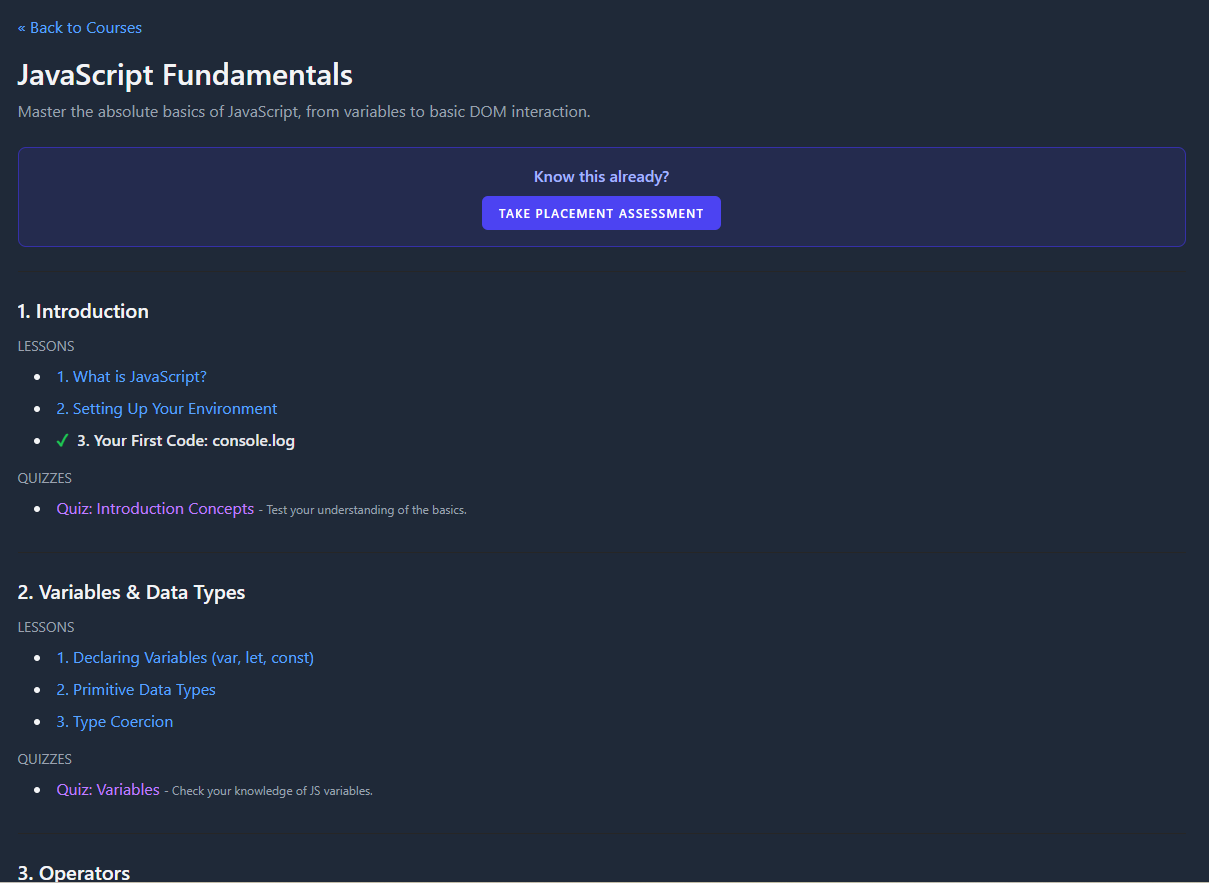
\includegraphics[scale=0.4]{images/module_example.png}
          \caption{Επισκόπηση ενός κύκλου μαθημάτων και των ενοτήτων του.}
          \label{fig:course_show_placeholder}
        \end{figure}
    \item \textbf{Περιεχόμενο Μαθημάτων (\eng{Lessons}):} Κάθε \eng{Lesson} περιλαμβάνει θεωρητικό υλικό, παραδείγματα κώδικα, και προαιρετικά οπτικοακουστικό υλικό (\eng{video\_embed\_html}).
        \begin{figure}[h!]
          \centering
          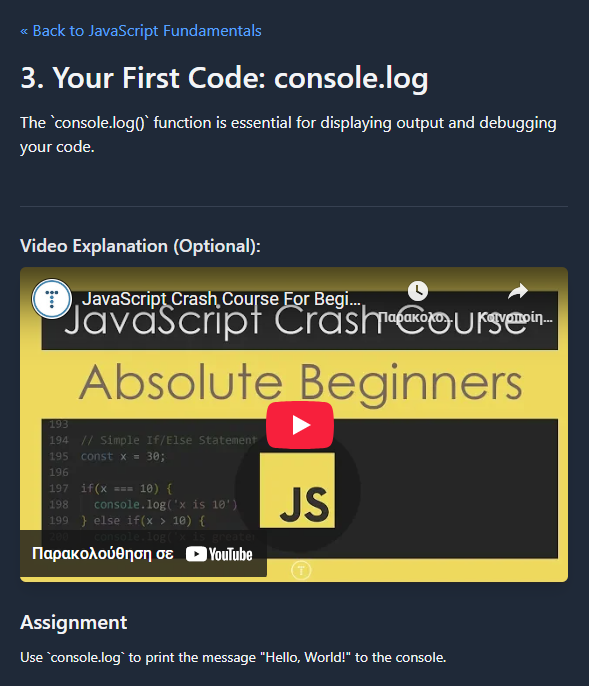
\includegraphics[scale=0.4]{images/lesson_content.png}
          \caption{Περιεχόμενο ενός μαθήματος.}
          \label{fig:lesson_content_placeholder}
        \end{figure}
    \item \textbf{Διαδραστικός Επεξεργαστής Κώδικα:} Κάθε \eng{Lesson} με άσκηση διαθέτει ενσωματωμένο \eng{code editor} (\eng{Monaco Editor}) για γραφή, τροποποίηση και \eng{client-side} εκτέλεση κώδικα.
    \item \textbf{Ασκήσεις Μαθημάτων:} Τα \eng{Lessons} μπορούν να περιλαμβάνουν \eng{assignment}. Η επιτυχής ολοκλήρωση (βάσει \eng{expected\_output}) μαρκάρει το μάθημα ως ολοκληρωμένο.
        \begin{figure}[h!]
          \centering
          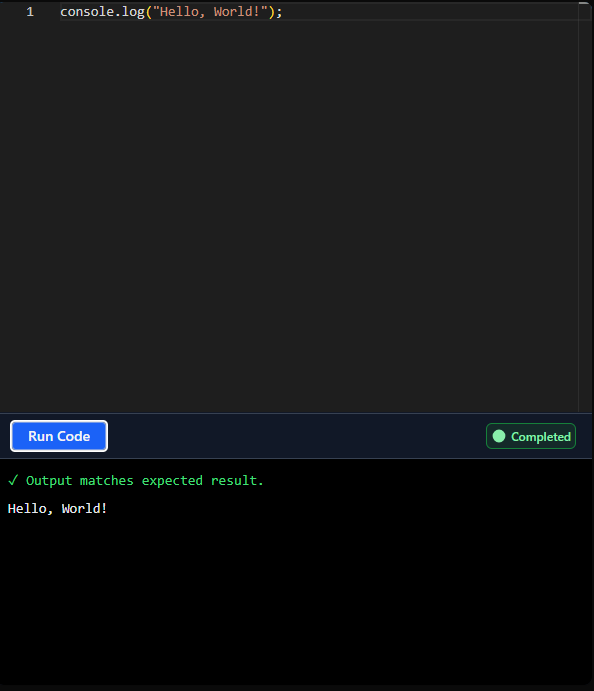
\includegraphics[scale=0.4]{images/lesson_editor.png}
          \caption{Διαδραστικός επεξεργαστής κώδικα και άσκηση μαθήματος.}
          \label{fig:lesson_editor_placeholder}
        \end{figure}
\end{itemize}

\subsubsection{Ερωτήσεις / Τεστ Αυτοαξιολόγησης}
\label{sec:test_autoaxiologisis}
Η εφαρμογή παρέχει σύστημα για \eng{quizzes} αυτοαξιολόγησης:
\begin{itemize}[leftmargin=*, noitemsep]
    \item \textbf{Τεστ ανά Ενότητα (\eng{Module Quizzes}):} Κάθε διδακτική υποενότητα (\eng{Module}) ενός \eng{Course} πρέπει να μπορεί να συνδέεται με ένα ή περισσότερα \eng{quizzes} που καλύπτουν το υλικό της συγκεκριμένης υποενότητας. Αυτά τα \eng{quizzes} βοηθούν τον χρήστη να ελέγξει την κατανόηση των εννοιών που μόλις διδάχθηκε.
    \item \textbf{Επαναληπτικά Τεστ:} Η εφαρμογή πρέπει να υποστηρίζει επαναληπτικά τεστ που συνδυάζουν ερωτήσεις από προηγούμενες ενότητες ή καλύπτουν το σύνολο ενός \eng{Course}. Συγκεκριμένα, υλοποιήθηκαν:
    \begin{itemize}[leftmargin=*, noitemsep]
        \item \textbf{Τελικό Επαναληπτικό \eng{Quiz} Κύκλου Μαθημάτων (\eng{Post-course Review Quiz}):} Στο τέλος κάθε \eng{Course}, ο χρήστης μπορεί να κάνει ένα επαναληπτικό \eng{quiz}. Αυτό το \eng{quiz} περιλαμβάνει δυναμικά ερωτήσεις στις οποίες ο χρήστης είχε απαντήσει λανθασμένα σε προηγούμενα \eng{module quizzes} του συγκεκριμένου \eng{course}, καθώς και τυχαίες νέες ερωτήσεις από το σύνολο του \eng{course}, για την ενίσχυση της μνήμης και της συνολικής κατανόησης.
        \item \textbf{Τυχαίο \eng{Quiz} Επανάληψης (\eng{Random Review Quiz}):} Τυχαίες ερωτήσεις από ολοκληρωμένα μαθήματα.
    \end{itemize}
    \item \textbf{Αξιολόγηση Αρχικού Επιπέδου (\eng{Pre-course Assessment Quiz}):} Για πρόταση σημείου εκκίνησης.
    \item \textbf{Ποικιλία Μορφών Ερωτήσεων:} Πολλαπλής Επιλογής, Σωστού/Λάθους, Συμπλήρωσης Κενού.
        \begin{figure}[h!]
          \centering
          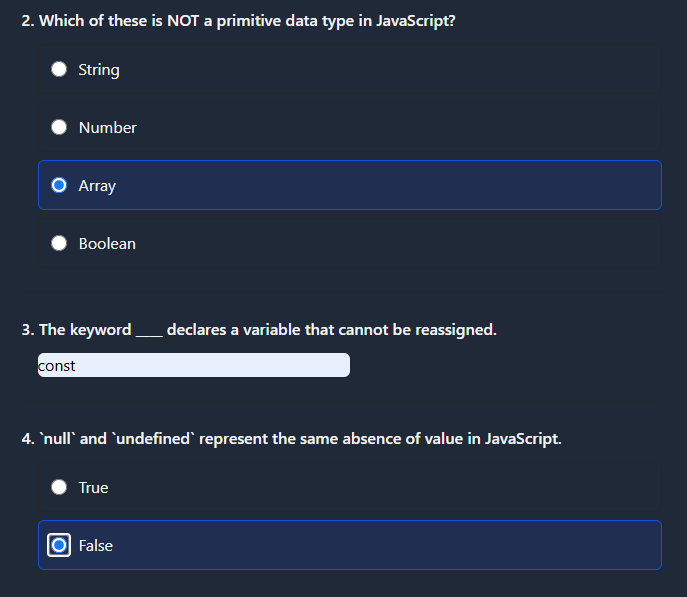
\includegraphics[scale=0.4]{images/question_types.png}
          \caption{Διεπαφή διεξαγωγής \eng{Quiz}.}
          \label{fig:quiz_interface_placeholder}
        \end{figure}
    \item \textbf{Διεπαφή Διεξαγωγής \eng{Quiz}:} Φιλικό περιβάλλον, άμεση ανατροφοδότηση (σκορ, σωστές/λανθασμένες απαντήσεις, εξηγήσεις).
    \item \textbf{Συστάσεις Βάσει Αποτελεσμάτων:} Πρόταση επανάληψης μαθημάτων και εξωτερικών πηγών.
        \begin{figure}[h!]
          \centering
          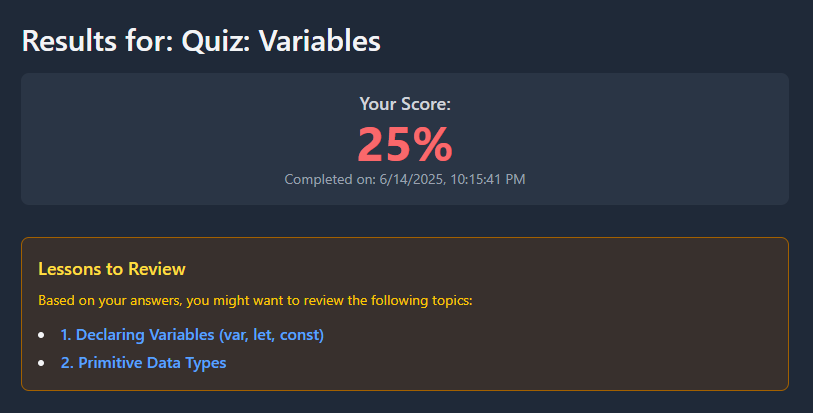
\includegraphics[scale=0.4]{images/quiz_results_recommendations.png}
          \caption{Αποτελέσματα \eng{Quiz} και προτάσεις επανάληψης.}
          \label{fig:quiz_results_placeholder}
        \end{figure}
\end{itemize}

\subsubsection{Αποθήκευση Στατιστικών Προόδου}
\label{sec:statistika_proodou}
Η εφαρμογή καταγράφει και αποθηκεύει δεδομένα προόδου:
\begin{itemize}[leftmargin=*, noitemsep]
    \item \textbf{Ολοκλήρωση Μαθημάτων (\eng{Lessons}):} Μέσω του πίνακα \eng{user\_progress} (\eng{user\_id, lesson\_id, completed\_at}).
    \item \textbf{Προσπάθειες και Αποτελέσματα \eng{Quiz}:} Στους πίνακες \eng{quiz\_attempts} (\eng{user\_id, quiz\_id (nullable), type, score, timestamps}) και \eng{quiz\_answers} (\eng{attempt\_id, question\_id, user\_answer, is\_correct}).
    \item \textbf{Δεδομένα Προφίλ και Προτιμήσεων Χρήστη:} Στον πίνακα \eng{users}.
\end{itemize}

\subsubsection{Προσαρμοσμένη Μάθηση (\eng{Adaptive Learning})}
\label{sec:adaptive_learning}
Η εφαρμογή στοχεύει στην παροχή μιας εμπειρίας προσαρμοσμένης μάθησης, όπου το εκπαιδευτικό περιεχόμενο και οι δραστηριότητες προσαρμόζονται δυναμικά στις επιδόσεις, τις προτιμήσεις και τις ανάγκες του κάθε μαθητή. Αυτό επιτυγχάνεται μέσω των παρακάτω μηχανισμών:
\begin{itemize}[leftmargin=*, noitemsep]
    \item \textbf{Αξιολόγηση Αρχικού Επιπέδου και Πρόταση Διαδρομής:} Μέσω του \eng{Pre-course Assessment Quiz} και του \eng{CourseAssessmentController}. Πριν την έναρξη ενός κύκλου μαθημάτων (\eng{Course}), ο χρήστης έχει τη δυνατότητα να συμμετάσχει σε ένα quiz αξιολόγησης αρχικού επιπέδου (\eng{Pre-course Assessment Quiz}). Βάσει των απαντήσεών του σε αυτό το \eng{quiz}, το σύστημα αξιολογεί την κατανόησή του σε θέματα που καλύπτονται στα αρχικά μαθήματα του \eng{course}. Εάν ο χρήστης επιδείξει επαρκή γνώση σε συγκεκριμένες ενότητες, η εφαρμογή του προτείνει να παρακάμψει τα αντίστοιχα αρχικά μαθήματα και να ξεκινήσει από ένα πιο προχωρημένο σημείο, αποφεύγοντας την επανάληψη υλικού που ήδη κατέχει.
        \begin{figure}[h!]
          \centering
          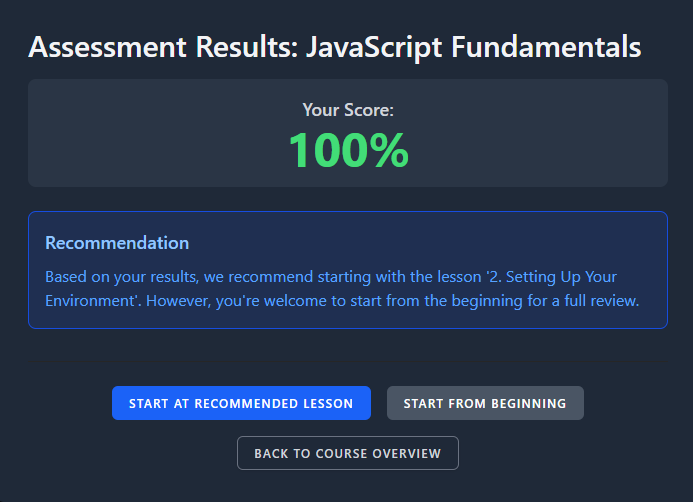
\includegraphics[scale=0.5]{images/assessment_result.png}
          \caption{Πρόταση μαθήματος μετά από αξιολόγηση αρχικού επιπέδου.}
          \label{fig:pre_course_result_placeholder}
        \end{figure}
    \item \textbf{Στοχευμένη Επανάληψη και Ενισχυτικό Υλικό:} Μέσω του \eng{Post-course Review Quiz}, του \eng{CourseReviewController} και του πίνακα \eng{external\_resources}.Μετά την ολοκλήρωση ενός τελικού επαναληπτικού \eng{quiz} ενός \eng{course} (\eng{Post-course Review Quiz}), εάν ο χρήστης εξακολουθεί να κάνει λάθη σε ερωτήσεις που αντιστοιχούν σε συγκεκριμένα μαθήματα, το σύστημα: Τον ανακατευθύνει ή του προτείνει να επισκεφθεί ξανά τα μαθήματα (\eng{lessons}) στα οποία παρουσίασε αδυναμίες. Παρέχει συνδέσμους προς επιλεγμένες εξωτερικές πηγές υλικού (π.χ. άρθρα, βίντεο, τεκμηρίωση) σχετικές με τα συγκεκριμένα μαθήματα, για περαιτέρω μελέτη και ενίσχυση της κατανόησης.
    \item \textbf{Προσαρμογή Παρουσίασης Περιεχομένου βάσει Μαθησιακού Στυλ:} Ο χρήστης μπορεί να δηλώσει στο \eng{dashboard} τον προτιμώμενο τρόπο μάθησης (π.χ. '\eng{visual}' για έμφαση σε οπτικό υλικό, '\eng{reading}' για έμφαση σε κείμενο). Στα μαθήματα που διαθέτουν τόσο κειμενικό όσο και οπτικοακουστικό υλικό (π.χ. ενσωματωμένα βίντεο), η εφαρμογή προσαρμόζει τη σειρά εμφάνισης αυτών των στοιχείων. Για παράδειγμα, ένας χρήστης που προτιμά οπτικό υλικό θα δει πρώτα το βίντεο και μετά το σχετικό κείμενο.
        \begin{figure}[h!]
          \centering
          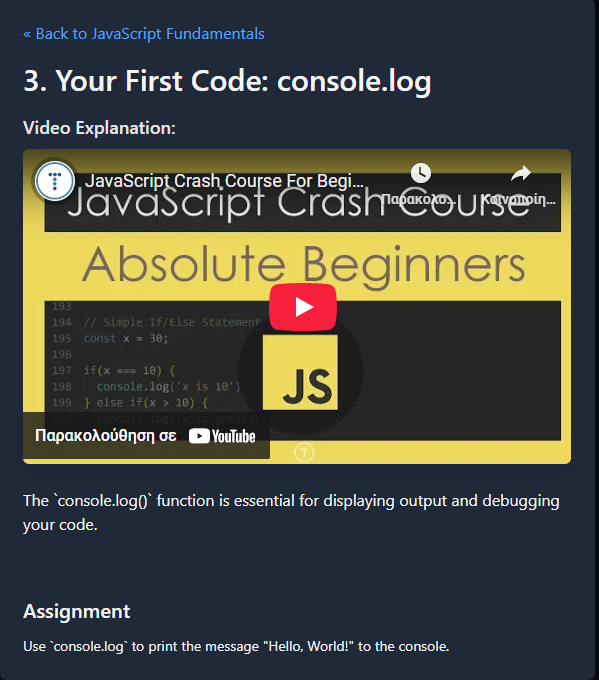
\includegraphics[scale=0.5]{images/visual_learner_lesson.png}
          \caption{Προσαρμογή εμφάνισης περιεχομένου βάσει μαθησιακού στυλ.}
          \label{fig:lesson_visual_placeholder}
        \end{figure}
    \item \textbf{Καθοδηγούμενα Μονοπάτια Μάθησης (\eng{Learning Paths}):} Ο χρήστης μπορεί να επιλέξει μια προκαθορισμένη μαθησιακή διαδρομή (\eng{Learning Path}) που αντιστοιχεί σε συγκεκριμένους εκπαιδευτικούς ή επαγγελματικούς στόχους (π.χ. \eng{"Frontend Developer Path", "Backend JavaScript Developer Path"}). Η εφαρμογή, βάσει της επιλεγμένης διαδρομής και της προόδου του χρήστη στα courses που την αποτελούν, προτείνει το επόμενο λογικό \eng{course} ή μάθημα για παρακολούθηση, παρέχοντας μια πιο δομημένη και καθοδηγούμενη πορεία μάθησης.
        \begin{figure}[h!]
          \centering
          \includegraphics[scale=0.4]{learning_path.png}
          \caption{Επιλεγμένη μαθησιακή διαδρομή και προτεινόμενο επόμενο μάθημα.}
          \label{fig:dashboard_path_placeholder}
        \end{figure}
    \item \textbf{Ρύθμιση Δυσκολίας Ασκήσεων/\eng{Quiz}:} Αν και δεν έχει υλοποιηθεί πλήρως δυναμική ρύθμιση δυσκολίας εντός ενός \eng{quiz}, η επιλογή των ερωτήσεων στα επαναληπτικά \eng{quizzes} (\eng{Post-course Review} και \eng{Random Review}) λαμβάνει υπόψη τις προηγούμενες επιδόσεις (εστιάζοντας σε λανθασμένες απαντήσεις), προσφέροντας έμμεσα μια μορφή προσαρμογής της δυσκολίας στην επανάληψη.
\end{itemize}

\subsubsection{Διαχείριση Χρήστη}
\label{sec:diacheirisi_xristi}
Παρέχονται βασικές λειτουργίες διαχείρισης λογαριασμού:
\begin{itemize}[leftmargin=*, noitemsep]
    \item Εγγραφή, Σύνδεση, Αποσύνδεση.
    \item Επεξεργασία Προφίλ (όνομα, \eng{email}, \eng{password}) και Μαθησιακών Προτιμήσεων (στυλ, \eng{path}) μέσω του \eng{Dashboard} και του \eng{UserPreferenceController}.
        \begin{figure}[h!]
          \centering
          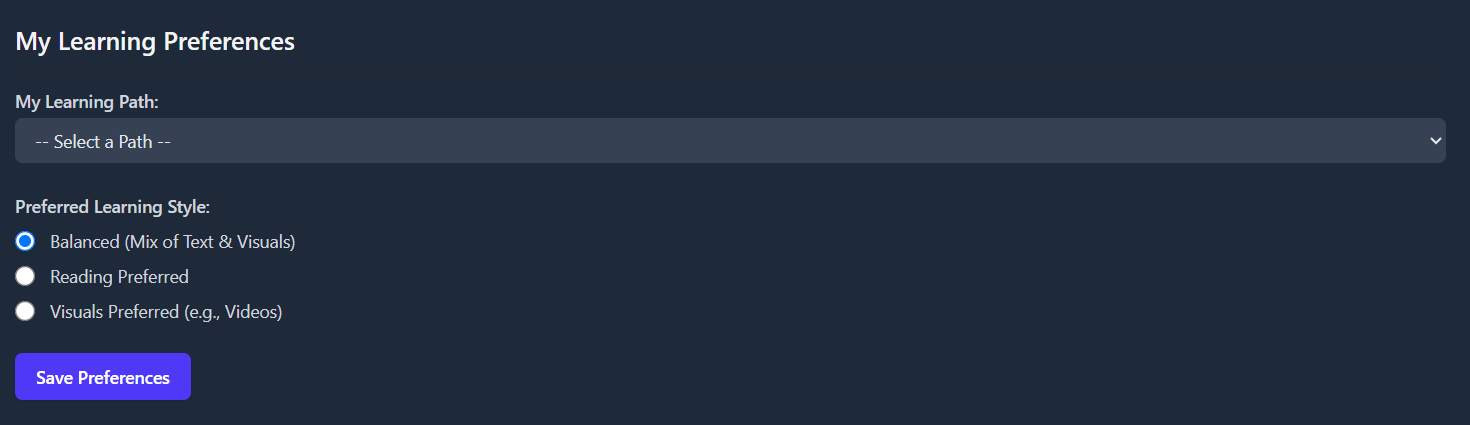
\includegraphics[scale=0.4]{preferences.png}
          \caption{Διαχείριση προτιμήσεων χρήστη στο \eng{Dashboard}.}
          \label{fig:dashboard_prefs_placeholder}
        \end{figure}
\end{itemize}

\subsubsection{Προβολή Αναφορών Προόδου}
\label{sec:anafores_proodou}
Οπτικοποιημένες αναφορές προόδου και στατιστικά στοιχεία:
\begin{itemize}[leftmargin=*, noitemsep]
    \item Μαθησιακό Σερί (\eng{Learning Streak}).
    \item Σύνολο Προσπαθειών σε \eng{Quiz}.
    \item Κατανομή Αποτελεσμάτων \eng{Quiz} (Πίτα).
    \item Γράφημα Ολοκληρωμένων Μαθημάτων ανά Ημέρα ("\eng{Contribution Graph}").
        \begin{figure}[h!]
          \centering
          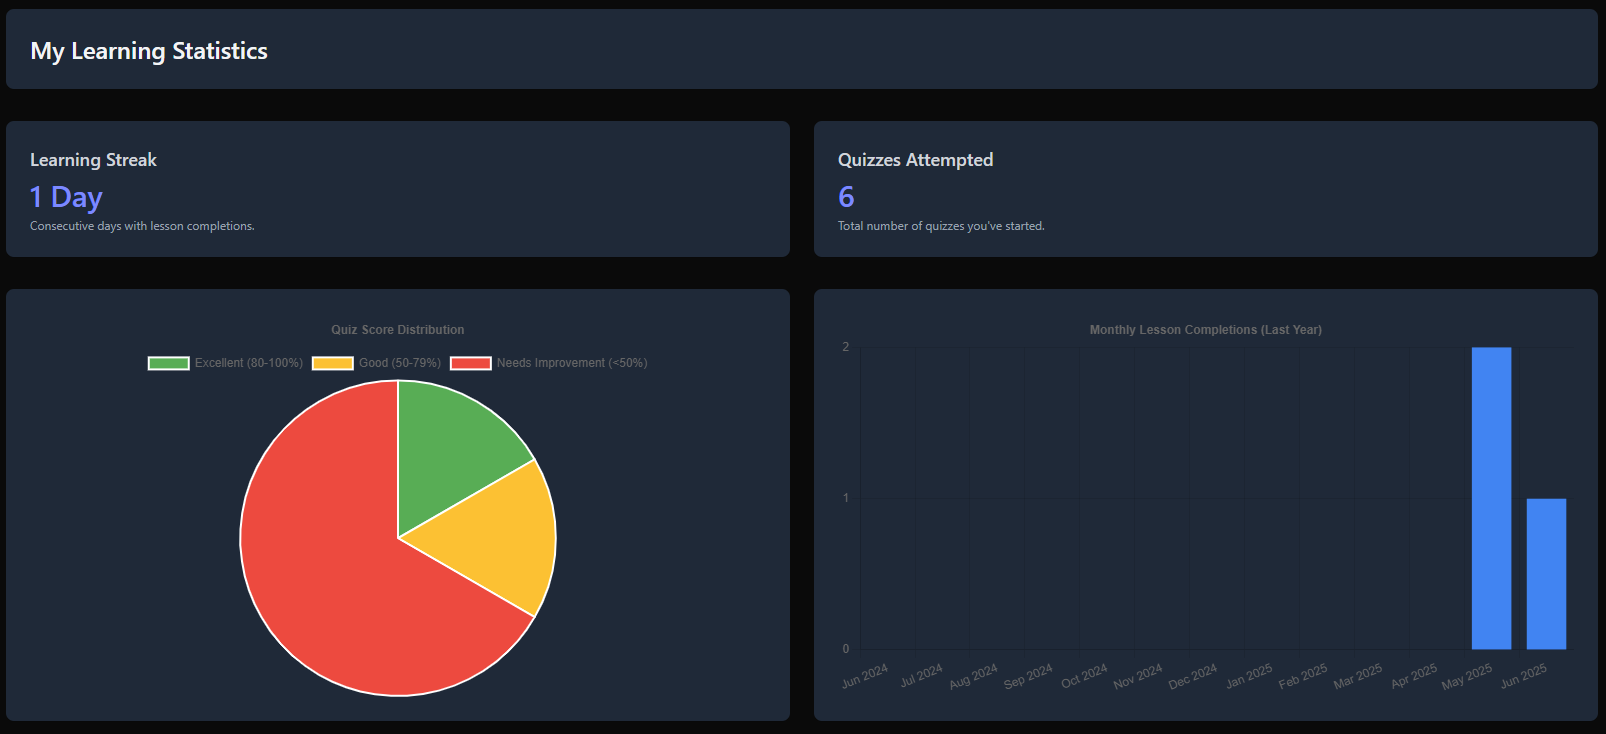
\includegraphics[scale=0.2]{statistics_page.png}
          \caption{Σελίδα στατιστικών προόδου χρήστη.}
          \label{fig:stats_page_placeholder}
        \end{figure}
\end{itemize}

\subsection{Μη Λειτουργικές Απαιτήσεις}
\label{sec:mi_leitourgikes_apaitiseis}
Πέραν των λειτουργιών, τέθηκαν και ποιοτικές απαιτήσεις:
\begin{itemize}[leftmargin=*, noitemsep]
    \item \textbf{Χρηστικότητα (\eng{Usability}):} Διαισθητικό και εύχρηστο περιβάλλον.
    \item \textbf{Απόδοση (\eng{Performance}):} Λογικοί χρόνοι φόρτωσης, άμεση απόκριση του \eng{editor}.
    \item \textbf{Ασφάλεια (\eng{Security}):} Προστασία δεδομένων χρήστη, \eng{client-side} εκτέλεση κώδικα από ελεγχόμενες πηγές περιεχομένου.
    \item \textbf{Συντηρησιμότητα (\eng{Maintainability}):} Οργανωμένος κώδικας.
    \item \textbf{Συμβατότητα (\eng{Compatibility}):} Λειτουργία σε σύγχρονους \eng{web browsers}.
\end{itemize}
% --- ΚΕΦΑΛΑΙΟ 3: ΣΧΕΔΙΑΣΜΟΣ ΣΥΣΤΗΜΑΤΟΣ ---
\section{Σχεδιασμός Συστήματος}
\label{sec:sxediasmos_systimatos}
Το παρόν κεφάλαιο περιγράφει τον σχεδιασμό του εκπαιδευτικού λογισμικού.

\subsection{Αρχιτεκτονική}
\label{sec:arxitektoniki}
Η αρχιτεκτονική της εφαρμογής βασίζεται σε ένα σύγχρονο \eng{web stack}, συνδυάζοντας την ισχύ του \eng{Laravel framework} για το \eng{backend} και την ευελιξία του \eng{Vue.js} με το \eng{Inertia.js} για ένα δυναμικό \eng{frontend}.
\textbf{Βασικά Συστατικά Αρχιτεκτονικής:}
\begin{enumerate}[leftmargin=*, noitemsep]
    \item \textbf{\eng{Client} (Πελάτης - Φυλλομετρητής Ιστού):} Ο χρήστης αλληλεπιδρά με την εφαρμογή μέσω ενός φυλλομετρητή ιστού (\eng{web browser}). Το \eng{frontend}, χτισμένο με \eng{Vue.js}, είναι υπεύθυνο για την παρουσίαση της διεπαφής χρήστη (\eng{UI}) και την αρχική διαχείριση των αλληλεπιδράσεων.

    \item \textbf{\eng{Web Server \& Backend} Εφαρμογή (\eng{Laravel}):} Ένας \eng{web server}φιλοξενεί την \eng{backend} εφαρμογή που έχει αναπτυχθεί με το \eng{PHP framework Laravel}.
    \begin{itemize}[leftmargin=+, noitemsep]
        \item Το \eng{Laravel} ακολουθεί την αρχιτεκτονική \eng{Model-View-Controller (MVC)}:
        \begin{itemize}[leftmargin=++, noitemsep]
            \item \textbf{\eng{Models}:} Αντιπροσωπεύουν τη δομή των δεδομένων και την αλληλεπίδραση με τη βάση δεδομένων (π.χ. \eng{User, Course, Lesson, Quiz}).
            \item \textbf{\eng{Views}:} Σε αυτή την εφαρμογή, οι "\eng{Views}" του \eng{Laravel} δεν είναι παραδοσιακά \eng{Blade templates} που παράγουν \eng{HTML}. Αντ' αυτού, οι \eng{Controllers} επιστρέφουν απαντήσεις \eng{Inertia.js}, οι οποίες ουσιαστικά ενημερώνουν το \eng{frontend} ποιο \eng{Vue component} να φορτώσει και τι δεδομένα (\eng{props}) να του περάσει.
            \item \textbf{\eng{Controllers}:} Διαχειρίζονται τα αιτήματα του χρήστη, αλληλεπιδρούν με τα \eng{Models} για την ανάκτηση ή αποθήκευση δεδομένων, και επιστρέφουν την κατάλληλη απόκριση (\eng{Inertia response}) στο \eng{frontend}.
        \end{itemize}
        \item Το \eng{backend} είναι επίσης υπεύθυνο για την αυθεντικοποίηση των χρηστών, την εξουσιοδότηση, την επικύρωση των δεδομένων και τη συνολική επιχειρησιακή λογική της εφαρμογής.
    \end{itemize}

    \item \textbf{Βάση Δεδομένων:} Μια σχεσιακή βάση δεδομένων (\eng{SQLite}) χρησιμοποιείται για την αποθήκευση όλων των μόνιμων δεδομένων της εφαρμογής, όπως πληροφορίες χρηστών, περιεχόμενο μαθημάτων, πρόοδο χρηστών, και αποτελέσματα \eng{quiz}. Το \eng{Laravel Eloquent ORM} χρησιμοποιείται για την εύκολη αλληλεπίδραση με τη βάση δεδομένων.

    \item \textbf{\eng{Inertia.js}:} Το \eng{Inertia.js} λειτουργεί ως "κόλλα" μεταξύ του \eng{Laravel backend} και του \eng{Vue.js frontend}. Επιτρέπει την ανάπτυξη σύγχρονων, \eng{single-page application (SPA)} εμπειριών χωρίς την πολυπλοκότητα της δημιουργίας ενός ξεχωριστού \eng{API}. Όταν ο χρήστης πλοηγείται, το \eng{Inertia} κάνει αιτήματα \eng{XHR} στο \eng{backend}, και το \eng{backend} επιστρέφει \eng{JSON} που περιλαμβάνει το όνομα του \eng{Vue component} που πρέπει να φορτωθεί και τα δεδομένα (\eng{props}) που χρειάζεται. Το \eng{routing} γίνεται κυρίως από το \eng{Laravel}.
\end{enumerate}

\textbf{Ροή Δεδομένων (Υψηλού Επιπέδου):}
\begin{enumerate}[leftmargin=*, noitemsep]
    \item Ο χρήστης αλληλεπιδρά με το \eng{Vue.js component} στον \eng{browser} του (π.χ. κλικάρει ένα \eng{link} για ένα μάθημα).
    \item Το \eng{Inertia.js} υποβάλλει ένα αίτημα (\eng{request}) στον \eng{Laravel server}.
    \item Το αντίστοιχο \eng{Route} στο \eng{Laravel} ενεργοποιεί τον κατάλληλο \eng{Controller}.
    \item Ο \eng{Controller} επεξεργάζεται το αίτημα, αλληλεπιδρά με τα \eng{Models} για να πάρει δεδομένα από τη Βάση Δεδομένων.
    \item Ο \eng{Controller} επιστρέφει ένα \eng{Inertia Response}, το οποίο περιέχει το όνομα του \eng{Vue page component} και τα δεδομένα (\eng{props}) που χρειάζεται.
    \item Το \eng{Inertia.js} στο \eng{frontend} λαμβάνει την απάντηση, φορτώνει δυναμικά το νέο \eng{Vue component} (ή ενημερώνει το υπάρχον) με τα νέα \eng{props}, ενημερώνοντας το \eng{UI} χωρίς πλήρη επαναφόρτωση της σελίδας.
\end{enumerate}

\begin{figure}[h!]
  \centering
  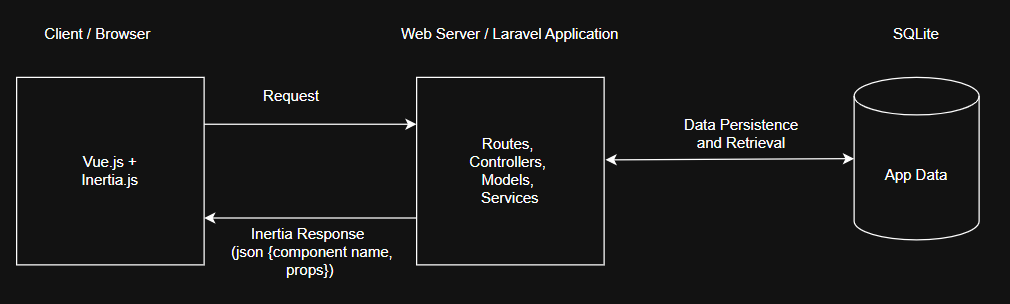
\includegraphics[scale=0.6]{architecture.png}
  \caption{Υψηλού Επιπέδου Αρχιτεκτονική Συστήματος.}
  \label{fig:arch_diag_placeholder_detailed}
\end{figure}

\subsection{Σχεδιασμός Βάσης Δεδομένων}
\label{sec:sxediasmos_bd_detailed}
Ο σχεδιασμός της βάσης δεδομένων αποτελεί θεμελιώδες τμήμα της εφαρμογής, καθώς είναι υπεύθυνος για την αποθήκευση και οργάνωση όλων των πληροφοριών που απαιτούνται για τη λειτουργία του εκπαιδευτικού λογισμικού. Χρησιμοποιήθηκε μια σχεσιακή βάση δεδομένων (\eng{SQLite} για την ανάπτυξη), και η αλληλεπίδραση με αυτήν γίνεται μέσω του \eng{Laravel Eloquent ORM}, το οποίο αντιστοιχίζει τους πίνακες της βάσης σε αντικείμενα (\eng{Models}).

Παρακάτω περιγράφονται οι κύριοι πίνακες (μοντέλα) της βάσης δεδομένων και οι μεταξύ τους σχέσεις.

\begin{figure}[h!]
  \centering
  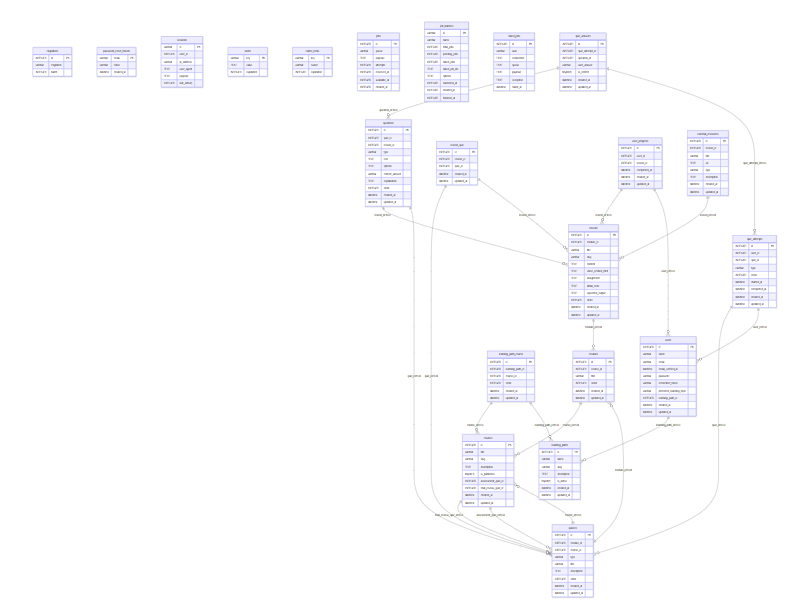
\includegraphics[scale=0.5]{erd.png}
  \caption{Διάγραμμα Σχήματος Βάσης Δεδομένων (\eng{ERD}).}
  \label{fig:erd_placeholder_detailed}
\end{figure}
\clearpage

\textbf{Περιγραφή Πινάκων (Μοντέλων):}

\begin{enumerate}[leftmargin=*, label=\arabic*., wide, labelwidth=!, labelindent=0pt, itemsep=1ex]
    \item \textbf{\texttt{\eng{users}} (Χρήστες):}
        \begin{itemize}[leftmargin=1.5em, noitemsep]
            \item \textit{Περιγραφή:} Αποθηκεύει πληροφορίες για τους εγγεγραμμένους χρήστες της πλατφόρμας.
            \item \textit{Βασικά Πεδία:} \texttt{\eng{id (PK)}}, \texttt{\eng{name}}, \texttt{\eng{email (unique)}}, \texttt{\eng{password (hashed)}}, \texttt{\eng{email\_verified\_at}}, \texttt{\eng{preferred\_learning\_style} (\eng{enum: 'reading', 'visual')}}, \texttt{\eng{learning\_path\_id (FK to learning\_paths, nullable)}}, \texttt{\eng{remember\_token}}, \texttt{\eng{timestamp}}.
            \item \textit{Σχέσεις:}
            \begin{itemize}[leftmargin=1.5em, noitemsep]
                \item Ένας χρήστης έχει πολλές εγγραφές προόδου (\eng{one-to-many with user\_progress}).
                \item Ένας χρήστης έχει πολλές προσπάθειες \eng{quiz (one-to-many with quiz\_attempts)}.
                \item Ένας χρήστης ανήκει σε μία μαθησιακή διαδρομή (\eng{many-to-one with learning\_paths}).
            \end{itemize}
        \end{itemize}

    \item \textbf{\texttt{\eng{learning\_paths}} (Μαθησιακές Διαδρομές):}
        \begin{itemize}[leftmargin=1.5em, noitemsep]
            \item \textit{Περιγραφή:} Καθορίζει προκαθορισμένες ακολουθίες μαθημάτων για συγκεκριμένους μαθησιακούς στόχους.
            \item \textit{Βασικά Πεδία:} \texttt{\eng{id (PK)}}, \texttt{\eng{name}}, \texttt{\eng{slug (unique)}}, \texttt{\eng{description}}, \texttt{\eng{is\_active}}, \texttt{\eng{timestamp}}.
            \item \textit{Σχέσεις:}
            \begin{itemize}[leftmargin=1.5em, noitemsep]
                \item Μία μαθησιακή διαδρομή έχει πολλούς χρήστες (\eng{one-to-many with users}).
                \item Μία μαθησιακή διαδρομή έχει πολλούς κύκλους μαθημάτων (\eng{many-to-many with courses} μέσω του πίνακα \texttt{\eng{learning\_path\_course}}).
            \end{itemize}
        \end{itemize}

    \item \textbf{\texttt{\eng{courses}} (Κύκλοι Μαθημάτων):}
        \begin{itemize}[leftmargin=1.5em, noitemsep]
            \item \textit{Περιγραφή:} Αντιπροσωπεύει ένα ολοκληρωμένο σύνολο διδακτικού υλικού για ένα ευρύτερο θέμα (π.χ., "\eng{JavaScript Fundamentals}").
            \item \textit{Βασικά Πεδία:} \texttt{\eng{id (PK)}}, \texttt{\eng{title}}, \texttt{\eng{slug (unique)}}, \texttt{\eng{description}}, \texttt{\eng{is\_published}}, \texttt{\eng{assessment\_quiz\_id} (\eng{FK} to \eng{quizzes, nullable})}, \texttt{\eng{final\_review\_quiz\_id (FK to quizzes, nullable)}}, \texttt{\eng{timestamp}}.
            \item \textit{Σχέσεις:}
            \begin{itemize}[leftmargin=1.5em, noitemsep]
                \item Ένας κύκλος μαθημάτων έχει πολλές ενότητες (\eng{one-to-many with modules}).
                \item Ένας κύκλος μαθημάτων ανήκει σε ένα (προαιρετικό) \eng{quiz} αξιολόγησης (\eng{many-to-one with quizzes}).
                \item Ένας κύκλος μαθημάτων ανήκει σε ένα (προαιρετικό) \eng{quiz} τελικής επανάληψης (\eng{many-to-one with quizzes}).
                \item Ένας κύκλος μαθημάτων ανήκει σε πολλές μαθησιακές διαδρομές (\eng{many-to-many with learning\_paths} μέσω του πίνακα \texttt{\eng{learning\_path\_course}}).
            \end{itemize}
        \end{itemize}

    \item \textbf{\texttt{\eng{modules}} (Ενότητες):}
        \begin{itemize}[leftmargin=1.5em, noitemsep]
            \item \textit{Περιγραφή:} Υποενότητες ενός \eng{Course}, ομαδοποιούν σχετικά μαθήματα.
            \item \textit{Βασικά Πεδία:} \texttt{\eng{id (PK)}}, \texttt{\eng{course\_id (FK)}}, \texttt{\eng{title}}, \texttt{\eng{order}}, \texttt{\eng{timestamp}}.
            \item \textit{Σχέσεις:}
            \begin{itemize}[leftmargin=1.5em, noitemsep]
                \item Μία ενότητα ανήκει σε έναν κύκλο μαθημάτων (\eng{many-to-one with courses}).
                \item Μία ενότητα έχει πολλά μαθήματα (\eng{one-to-many with lessons}).
                \item Μία ενότητα έχει πολλά \eng{quizzes (one-to-many with quizzes} - για τα \eng{module quizzes}).
            \end{itemize}
        \end{itemize}

    \item \textbf{\texttt{\eng{lessons}} (Μαθήματα):}
        \begin{itemize}[leftmargin=1.5em, noitemsep]
            \item \textit{Περιγραφή:} Η μικρότερη διδακτική μονάδα, περιέχει το εκπαιδευτικό υλικό και τις ασκήσεις.
            \item \textit{Βασικά Πεδία:} \texttt{\eng{id (PK)}}, \texttt{\eng{module\_id (FK)}}, \texttt{\eng{title}}, \texttt{\eng{slug (unique)}}, \texttt{\eng{content (HTML/Markdown)}}, \texttt{\eng{assignment}}, \texttt{\eng{initial\_code}}, \texttt{\eng{expected\_output}}, \texttt{\eng{video\_embed\_html (nullable)}}, \texttt{\eng{order}}, \texttt{\eng{timestamp}}.
            \item \textit{Σχέσεις:}
            \begin{itemize}[leftmargin=1.5em, noitemsep]
                \item Ένα μάθημα ανήκει σε μία ενότητα (\eng{many-to-one with modules}).
                \item Ένα μάθημα έχει πολλές εγγραφές προόδου χρηστών (\eng{one-to-many with user\_progress}).
                \item Ένα μάθημα έχει πολλές εξωτερικές πηγές (\eng{one-to-many with external\_resources}).
                \item Ένα μάθημα μπορεί να σχετίζεται με πολλές ερωτήσεις \eng{quiz (many-to-one from questions}).
            \end{itemize}
        \end{itemize}

    \item \textbf{\texttt{\eng{quizzes}}:}
        \begin{itemize}[leftmargin=1.5em, noitemsep]
            \item \textit{Περιγραφή:} Αντιπροσωπεύει ένα σύνολο ερωτήσεων για αξιολόγηση.
            \item \textit{Βασικά Πεδία:} \texttt{\eng{id (PK)}}, \texttt{\eng{type (enum: 'assessment', 'module', 'final\_review')}}, \texttt{\eng{module\_id (FK, nullable)}}, \texttt{\eng{title}}, \texttt{\eng{description}}, \texttt{\eng{order}}, \texttt{\eng{timestamp}}.
            \item \textit{Σχέσεις:}
            \begin{itemize}[leftmargin=1.5em, noitemsep]
                \item Ένα \eng{quiz} έχει πολλές ερωτήσεις (\eng{one-to-many with questions}).
                \item Ένα \eng{quiz} έχει πολλές προσπάθειες από χρήστες (\eng{one-to-many with quiz\_attempts}).
                \item Ένα \eng{quiz} (τύπου '\eng{module}') ανήκει σε μία ενότητα (\eng{many-to-one with modules}).
                \item Ένα \eng{quiz} (τύπου '\eng{assessment}' ή '\eng{final\_review}') μπορεί να συνδέεται με ένα \eng{course} (\eng{one-to-one relationships from courses}).
            \end{itemize}
        \end{itemize}

    \item \textbf{\texttt{\eng{questions}} (Ερωτήσεις):}
        \begin{itemize}[leftmargin=1.5em, noitemsep]
            \item \textit{Περιγραφή:} Μια μεμονωμένη ερώτηση ενός \eng{quiz}.
            \item \textit{Βασικά Πεδία:} \texttt{\eng{id (PK)}}, \texttt{\eng{quiz\_id (FK)}}, \texttt{\eng{lesson\_id (FK, nullable)}}, \texttt{\eng{type (enum: 'multiple\_choice', 'true\_false', 'fill\_blank')}}, \texttt{\eng{text}}, \texttt{\eng{options (JSON, nullable)}}, \texttt{\eng{correct\_answer}}, \texttt{\eng{explanation}}, \texttt{\eng{order}}, \texttt{\eng{timestamp}}.
            \item \textit{Σχέσεις:}
            \begin{itemize}[leftmargin=1.5em, noitemsep]
                \item Μία ερώτηση ανήκει σε ένα \eng{quiz (many-to-one with quizzes)}.
                \item Μία ερώτηση μπορεί να σχετίζεται με ένα μάθημα (\eng{many-to-one with lessons}).
            \end{itemize}
        \end{itemize}

    \item \textbf{\texttt{\eng{user\_progress}} (Πρόοδος Χρήστη):}
        \begin{itemize}[leftmargin=1.5em, noitemsep]
            \item \textit{Περιγραφή:} Καταγράφει την ολοκλήρωση μαθημάτων από τους χρήστες.
            \item \textit{Βασικά Πεδία:} \texttt{\eng{id (PK)}}, \texttt{\eng{user\_id (FK)}}, \texttt{\eng{lesson\_id (FK)}}, \texttt{\eng{completed\_at}}, \texttt{\eng{timestamp}}.
            \item \textit{Σχέσεις:}
            \begin{itemize}[leftmargin=1.5em, noitemsep]
                \item Ανήκει σε έναν χρήστη (\eng{many-to-one with users}).
                \item Ανήκει σε ένα μάθημα (\eng{many-to-one with lessons}).
            \end{itemize}
            \item \textit{Περιορισμός:} Μοναδικό ζεύγος (\texttt{\eng{user\_id, lesson\_id}}).
        \end{itemize}

    \item \textbf{\texttt{\eng{quiz\_attempts}} (Προσπάθειες \eng{Quiz}):}
        \begin{itemize}[leftmargin=1.5em, noitemsep]
            \item \textit{Περιγραφή:} Καταγράφει κάθε προσπάθεια ενός χρήστη σε ένα \eng{quiz}.
            \item \textit{Βασικά Πεδία:} \texttt{\eng{id (PK)}}, \texttt{\eng{user\_id (FK)}}, \texttt{\eng{quiz\_id (FK, nullable)}}, \texttt{\eng{type (string: 'standard', 'random', 'final\_review')}}, \texttt{\eng{score}}, \texttt{\eng{started\_at}}, \texttt{\eng{completed\_at}}, \texttt{\eng{timestamp}}.
            \item \textit{Σχέσεις:}
            \begin{itemize}[leftmargin=1.5em, noitemsep]
                \item Ανήκει σε έναν χρήστη (\eng{many-to-one with users}).
                \item Ανήκει σε ένα \eng{quiz (many-to-one with quizzes}, αν \texttt{quiz\_id not null}).
                \item Μία προσπάθεια έχει πολλές απαντήσεις (\eng{one-to-many with quiz\_answers}).
            \end{itemize}
        \end{itemize}

    \item \textbf{\texttt{\eng{quiz\_answers}} (Απαντήσεις \eng{Quiz}):}
        \begin{itemize}[leftmargin=1.5em, noitemsep]
            \item \textit{Περιγραφή:} Αποθηκεύει τη συγκεκριμένη απάντηση ενός χρήστη σε μια ερώτηση μιας προσπάθειας \eng{quiz}.
            \item \textit{Βασικά Πεδία:} \texttt{\eng{id (PK)}}, \texttt{\eng{quiz\_attempt\_id (FK)}}, \texttt{\eng{question\_id (FK)}}, \texttt{\eng{user\_answer}}, \texttt{\eng{is\_correct}}, \texttt{\eng{timestamp}}.
            \item \textit{Σχέσεις:}
            \begin{itemize}[leftmargin=1.5em, noitemsep]
                \item Ανήκει σε μία προσπάθεια \eng{quiz (many-to-one with quiz\_attempts)}.
                \item Ανήκει σε μία ερώτηση (\eng{many-to-one with questions}).
            \end{itemize}
            \item \textit{Περιορισμός:} Μοναδικό ζεύγος (\texttt{\eng{quiz\_attempt\_id, question\_id}}).
        \end{itemize}

    \item \textbf{\texttt{\eng{external\_resources}} (Εξωτερικές Πηγές):}
        \begin{itemize}[leftmargin=1.5em, noitemsep]
            \item \textit{Περιγραφή:} Σύνδεσμοι και πληροφορίες για επιπλέον υλικό μελέτης.
            \item \textit{Βασικά Πεδία:} \texttt{\eng{id (PK)}}, \texttt{\eng{lesson\_id (FK)}}, \texttt{\eng{title}}, \texttt{\eng{url}}, \texttt{\eng{type (enum)}}, \texttt{\eng{description}}, \texttt{\eng{timestamps}}.
            \item \textit{Σχέσεις:}
            \begin{itemize}[leftmargin=1.5em, noitemsep]
                \item Ανήκει σε ένα μάθημα (\eng{many-to-one with lessons}).
            \end{itemize}
        \end{itemize}

    \item \textbf{\texttt{\eng{learning\_path\_course}} (Πίνακας Συσχέτισης):}
        \begin{itemize}[leftmargin=1.5em, noitemsep]
            \item \textit{Περιγραφή:} Συνδέει τις μαθησιακές διαδρομές με τους κύκλους μαθημάτων, καθορίζοντας τη σειρά τους.
            \item \textit{Βασικά Πεδία:} \texttt{\eng{id (PK)}}, \texttt{\eng{learning\_path\_id (FK)}}, \texttt{\eng{course\_id (FK)}}, \texttt{\eng{order}}.
            \item \textit{Περιορισμός:} Μοναδικό ζεύγος (\texttt{\eng{learning\_path\_id, course\_id}}).
        \end{itemize}
\end{enumerate}

\subsection{Σχεδιασμός Λειτουργιών Εξατομίκευσης}
\label{sec:logiki_exatomikeusis}
Η εφαρμογή ενσωματώνει διάφορους μηχανισμούς για την παροχή μιας εξατομικευμένης μαθησιακής εμπειρίας. Ο σχεδιασμός αυτών των λειτουργιών βασίζεται στην ανάλυση των δεδομένων προόδου και των προτιμήσεων του χρήστη. Παρακάτω περιγράφεται η βασική λογική πίσω από κάθε χαρακτηριστικό εξατομίκευσης:

\begin{enumerate}[leftmargin=*, label=\arabic*., wide, labelwidth=!, labelindent=0pt, itemsep=1ex]
    \item \textbf{Πρόταση Παράκαμψης Μαθημάτων (\eng{Pre-course Assessment}):}
        \begin{itemize}[leftmargin=1.5em, noitemsep]
            \item \textit{Ενεργοποίηση:} Όταν ο χρήστης επιλέγει να ξεκινήσει ένα \eng{Course} που διαθέτει \eng{Quiz} Αξιολόγησης Αρχικού Επιπέδου (\texttt{\eng{assessment\_quiz}}).
            \item \textit{Διαδικασία:}
            \begin{enumerate}[leftmargin=1.5em, label=\alph*), noitemsep]
                \item Ο χρήστης ολοκληρώνει το \eng{Assessment Quiz}.
                \item Ο \texttt{\eng{CourseAssessmentController}} λαμβάνει τις απαντήσεις.
                \item Για κάθε ερώτηση του \eng{quiz} (οι οποίες είναι συνδεδεμένες με συγκεκριμένα αρχικά \eng{lessons} του \eng{Course} μέσω του πεδίου \texttt{\eng{lesson\_id}} στον πίνακα \texttt{\eng{questions}}), ελέγχεται η ορθότητα της απάντησης.
                \item Συγκεντρώνονται τα αποτελέσματα ανά \texttt{\eng{lesson\_id}}. Υπολογίζεται ένα ποσοστό επιτυχίας για τις ερωτήσεις που αντιστοιχούν σε κάθε αρχικό \eng{lesson}.
                \item Το σύστημα διατρέχει τα \eng{lessons} του \eng{Course} με τη σειρά.
                \item Εάν ένα \eng{lesson} δεν είχε ερωτήσεις στο \eng{assessment quiz}, ή εάν ο χρήστης δεν πέτυχε ένα προκαθορισμένο ποσοστό επιτυχίας (π.χ., 80\%) στις ερωτήσεις που αντιστοιχούσαν σε αυτό, τότε αυτό το \eng{lesson} προτείνεται ως το σημείο εκκίνησης.
                \item Εάν ο χρήστης περάσει επιτυχώς τις ερωτήσεις για όλα τα αρχικά \eng{lessons} που καλύπτονταν από το \eng{assessment}, του προτείνεται να ξεκινήσει από το πρώτο \eng{lesson} (ως ασφαλής επιλογή) ή ενημερώνεται ότι φαίνεται να κατέχει το υλικό και μπορεί να προχωρήσει σε πιο προχωρημένες ενότητες.
            \end{itemize}
            \item \textit{Αποτέλεσμα:} Ο χρήστης λαμβάνει μια προσωποποιημένη πρόταση για το από ποιο μάθημα θα μπορούσε να ξεκινήσει, μαζί με την επιλογή να αγνοήσει την πρόταση και να ξεκινήσει από την αρχή.
            \begin{figure}[h!]
              \centering
              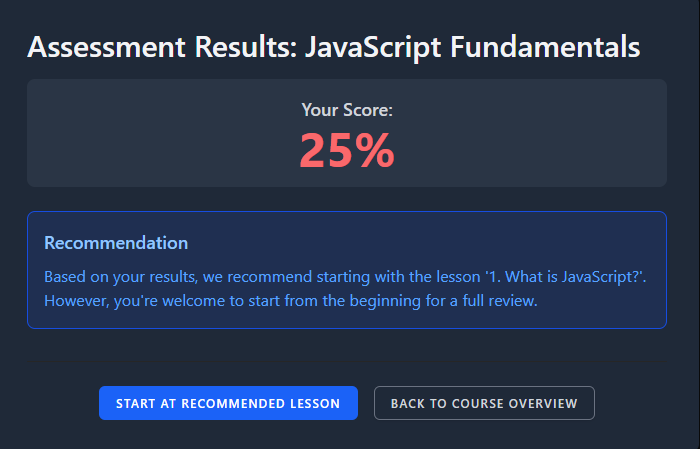
\includegraphics[scale=0.4]{images/assessment_result2.png}
              \caption{Πρόταση μαθήματος βάσει αξιολόγησης αρχικού επιπέδου.}
              \label{fig:pre_course_recom_placeholder}
            \end{figure}
        \end{itemize}

    \item \textbf{Πρόταση Ενισχυτικού Υλικού (\eng{Post-course Review Quiz}):}
        \begin{itemize}[leftmargin=1.5em, noitemsep]
            \item \textit{Ενεργοποίηση:} Μετά την ολοκλήρωση του Τελικού Επαναληπτικού \eng{Quiz} ενός \eng{Course}.
            \item \textit{Διαδικασία:}
            \begin{enumerate}[leftmargin=1.5em, label=\alph*), noitemsep]
                \item Ο χρήστης ολοκληρώνει το \eng{Post-course Review Quiz}.
                \item Ο \texttt{\eng{CourseReviewController}} λαμβάνει και βαθμολογεί τις απαντήσεις.
                \item Για κάθε λανθασμένη απάντηση, εντοπίζεται το \texttt{\eng{lesson\_id}} με το οποίο σχετίζεται η ερώτηση.
                \item Για κάθε τέτοιο \eng{lesson}, ανακτώνται από τη βάση δεδομένων οι σχετικές εξωτερικές πηγές υλικού (\texttt{\eng{external\_resources}}).
            \end{enumerate}
            \item \textit{Αποτέλεσμα:} Στη σελίδα αποτελεσμάτων του \eng{quiz}, μαζί με τις σωστές/λανθασμένες απαντήσεις, ο χρήστης βλέπει μια λίστα με τα μαθήματα που χρειάζονται επανάληψη και, για καθένα από αυτά, προτεινόμενους συνδέσμους προς εξωτερικές πηγές (άρθρα, βίντεο, τεκμηρίωση) για περαιτέρω μελέτη.
            \begin{figure}[h!]
              \centering
              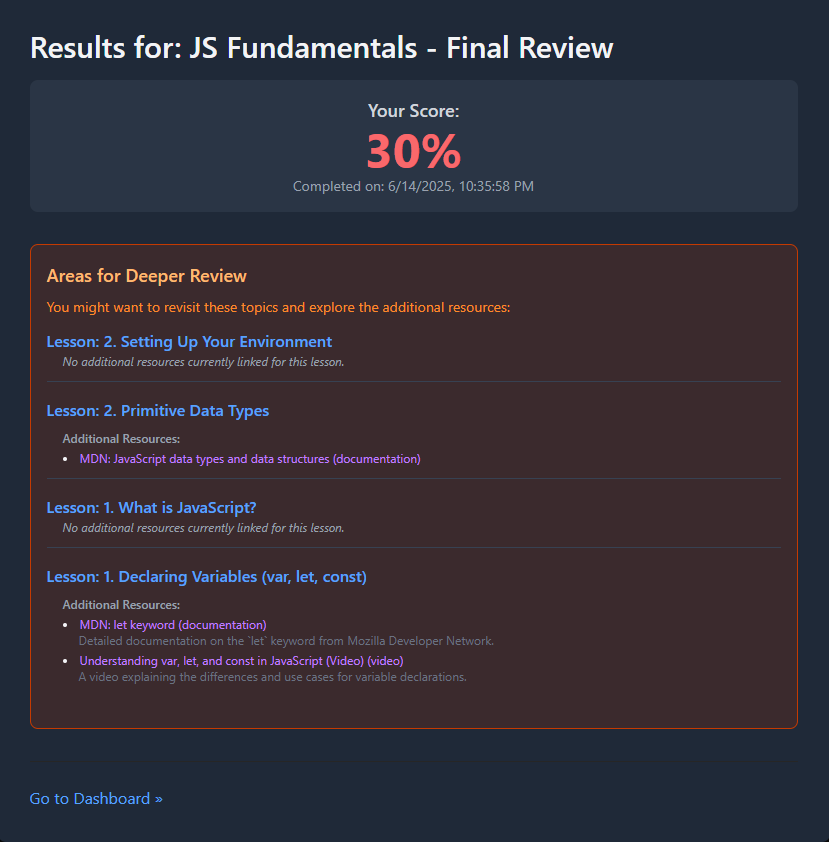
\includegraphics[scale=0.3]{images/final_review.png}
              \caption{Προτάσεις επανάληψης και ενισχυτικού υλικού.}
              \label{fig:post_course_resources_placeholder}
            \end{figure}
        \end{itemize}

    \item \textbf{Προσαρμογή Εμφάνισης Περιεχομένου (\eng{Visual vs. Reading Style}):}
        \begin{itemize}[leftmargin=1.5em, noitemsep]
            \item \textit{Ενεργοποίηση:} Ο χρήστης ορίζει την προτίμησή του (\texttt{\eng{preferred\_learning\_style}}) στο \eng{Dashboard}.
            \item \textit{Διαδικασία:}
            \begin{enumerate}[leftmargin=1.5em, label=\alph*), noitemsep]
                \item Η προτίμηση του χρήστη είναι διαθέσιμη στο \eng{frontend (Vue component lessons/Show.vue)} μέσω των \eng{global props} του \eng{Inertia}.
                \item Το \eng{component} ελέγχει την τιμή του \texttt{\eng{user.preferred\_learning\_style}} και την ύπαρξη ενσωματωμένου βίντεο (\texttt{\eng{lesson.video\_embed\_html}}).
                \item Εάν η προτίμηση είναι '\eng{visual}' και υπάρχει βίντεο, το μπλοκ του βίντεο εμφανίζεται πριν από το κειμενικό περιεχόμενο του μαθήματος.
                \item Σε αντίθετη περίπτωση (προτίμηση '\eng{reading}' ή δεν υπάρχει βίντεο), το κειμενικό περιεχόμενο εμφανίζεται πρώτο, και το βίντεο (αν υπάρχει) εμφανίζεται μετά, ως προαιρετικό.
            \end{enumerate}
            \item \textit{Αποτέλεσμα:} Η σειρά παρουσίασης των διαφορετικών τύπων περιεχομένου προσαρμόζεται στην προτίμηση του χρήστη, με στόχο την καλύτερη δυνατή εμπλοκή.
            \begin{figure}[h!]
              \centering
              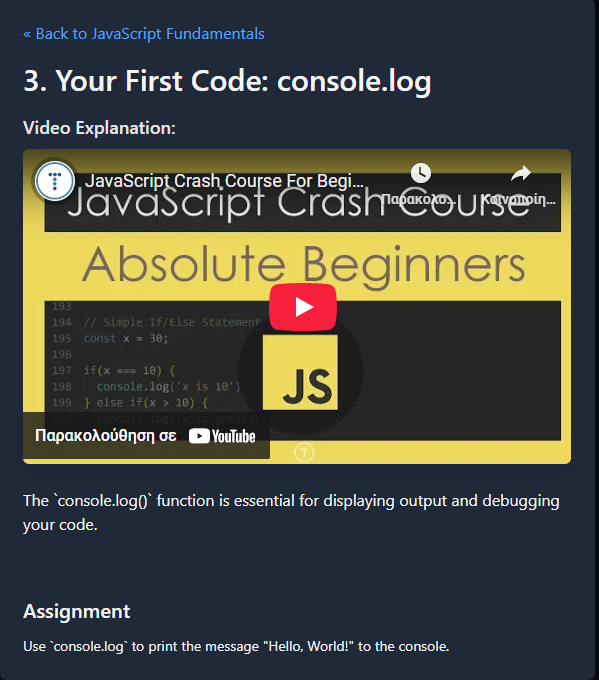
\includegraphics[scale=0.4]{images/visual_learner_lesson.png}
              \caption{Προσαρμογή εμφάνισης περιεχομένου.}
              \label{fig:lesson_visual_first_placeholder}
            \end{figure}
        \end{itemize}

    \item \textbf{Καθοδήγηση βάσει Μαθησιακού Στόχου (\eng{Learning Paths}):}
        \begin{itemize}[leftmargin=1.5em, noitemsep]
            \item \textit{Ενεργοποίηση:} Ο χρήστης επιλέγει μια Μαθησιακή Διαδρομή (\texttt{\eng{learning\_path}}) στο \eng{Dashboard}.
            \item \textit{Διαδικασία:}
            \begin{enumerate}[leftmargin=1.5em, label=\alph*), noitemsep]
                \item Η επιλεγμένη διαδρομή του χρήστη είναι γνωστή στο \eng{backend (DashboardController)}.
                \item Ο \eng{controller} ανακτά τα \eng{Courses} που ανήκουν σε αυτή τη διαδρομή, στη σωστή σειρά (βάσει του πεδίου \texttt{order} στον πίνακα \texttt{\eng{learning\_path\_course}}).
                \item Για κάθε \eng{Course} στη διαδρομή, ελέγχεται η πρόοδος του χρήστη (ολοκληρωμένα \eng{lessons} μέσω του \texttt{\eng{user\_progress}}).
                \item Το πρώτο \eng{Course} στη σειρά της διαδρομής για το οποίο ο χρήστης δεν έχει ολοκληρώσει όλα τα μαθήματα (ή ένα σημαντικό ποσοστό αυτών) προτείνεται ως το "Επόμενο Προτεινόμενο \eng{Course}".
                \item Αν όλα τα \eng{Courses} της διαδρομής έχουν ολοκληρωθεί, εμφανίζεται ένα μήνυμα επιτυχίας.
            \end{enumerate}
            \item \textit{Αποτέλεσμα:} Στο \eng{Dashboard}, ο χρήστης βλέπει την τρέχουσα μαθησιακή του διαδρομή και μια σαφή πρόταση για το ποιο \eng{course} να παρακολουθήσει στη συνέχεια, παρέχοντας δομή και κατεύθυνση.
            \begin{figure}[h!]
              \centering
              \includegraphics[scale=0.3]{images/learning_path.png}
              \caption{Καθοδήγηση μαθησιακής διαδρομής.}
              \label{fig:dashboard_path_suggestion_placeholder}
            \end{figure}
        \end{itemize}
\end{enumerate}

\subsection{Σημαντικά \eng{Components}}
\label{sec:simantika_components_detailed}
Η εφαρμογή δομείται γύρω από ένα σύνολο διακριτών \eng{components} στο \eng{backend} (κυρίως \eng{Laravel Controllers}) και στο \eng{frontend} (\eng{Vue Pages} και επαναχρησιμοποιήσιμα \eng{Vue Components}). Αυτή η προσέγγιση προάγει την οργάνωση, τη συντηρησιμότητα και την επεκτασιμότητα του κώδικα.

\subsubsection{\eng{Backend Components (Laravel Controllers)}}
\label{sec:backend_controllers_detailed}
Οι παρακάτω είναι οι κύριοι \eng{controllers} που διαχειρίζονται την επιχειρησιακή λογική της εφαρμογής στην πλευρά του \eng{server}:
\begin{itemize}[leftmargin=*, noitemsep]
    \item \textbf{\texttt{\eng{DashboardController}}:}
        \begin{itemize}[leftmargin=+, noitemsep]
            \item \textit{Ρόλος:} Υπεύθυνος για τη συγκέντρωση και παροχή των δεδομένων που απαιτούνται για την αρχική σελίδα (\eng{dashboard}) του συνδεδεμένου χρήστη. Αυτό περιλαμβάνει τις προτιμήσεις του χρήστη (\eng{learning path, learning style}), τις διαθέσιμες μαθησιακές διαδρομές, το επόμενο προτεινόμενο \eng{course} βάσει της επιλεγμένης διαδρομής, και το ιστορικό πρόσφατων προσπαθειών σε \eng{quizzes}.
        \end{itemize}
    \item \textbf{\texttt{\eng{CourseController}}:}
        \begin{itemize}[leftmargin=+, noitemsep]
            \item \textit{Ρόλος:} Διαχειρίζεται τις λειτουργίες που σχετίζονται με τους κύκλους μαθημάτων (\eng{Courses}).
            \item \textit{Βασικές Μέθοδοι:} \texttt{\eng{index()}} για την εμφάνιση λίστας όλων των δημοσιευμένων \eng{courses}, \texttt{\eng{show()}} για την εμφάνιση των λεπτομερειών ενός συγκεκριμένου \eng{course (modules, lessons, quizzes} ενότητας, \eng{link} για \eng{assessment/review}).
        \end{itemize}
    \item \textbf{\texttt{\eng{LessonController}}:}
        \begin{itemize}[leftmargin=+, noitemsep]
            \item \textit{Ρόλος:} Διαχειρίζεται την εμφάνιση των μεμονωμένων μαθημάτων (\eng{Lessons}).
            \item \textit{Βασικές Μέθοδοι:} \texttt{\eng{show()}} для την παρουσίαση του περιεχομένου ενός μαθήματος, της άσκησης, του αρχικού κώδικα και την προετοιμασία της διεπαφής με τον \eng{code editor}.
        \end{itemize}
    \item \textbf{\texttt{\eng{QuizController}}:}
        \begin{itemize}[leftmargin=+, noitemsep]
            \item \textit{Ρόλος:} Διαχειρίζεται τη διεξαγωγή των τυπικών \eng{quizzes (module quizzes)}.
            \item \textit{Βασικές Μέθοδοι:} \texttt{\eng{show()}} для την εμφάνιση των ερωτήσεων ενός \eng{quiz}, \texttt{\eng{submit()}} для την παραλαβή των απαντήσεων, τη βαθμολόγηση, την αποθήκευση της προσπάθειας (\eng{QuizAttempt} και \eng{QuizAnswer}) και την εμφάνιση των αποτελεσμάτων.
        \end{itemize}
    \item \textbf{\texttt{\eng{UserProgressController}}:}
        \begin{itemize}[leftmargin=+, noitemsep]
            \item \textit{Ρόλος:} Διαχειρίζεται την καταγραφή της προόδου του χρήστη.
            \item \textit{Βασικές Μέθοδοι:} \texttt{\eng{store()}} для την επισήμανση ενός μαθήματος (\eng{Lesson}) ως ολοκληρωμένου από τον χρήστη, συνήθως μετά την επιτυχή ολοκλήρωση της άσκησης κώδικα.
        \end{itemize}
    \item \textbf{\texttt{\eng{CourseAssessmentController}}:}
        \begin{itemize}[leftmargin=+, noitemsep]
            \item \textit{Ρόλος:} Διαχειρίζεται τα \eng{quizzes} αξιολόγησης αρχικού επιπέδου (\eng{Pre-course Assessment}).
            \item \textit{Βασικές Μέθοδοι:} \texttt{\eng{show()}} για την εμφάνιση του \eng{assessment quiz}, \texttt{\eng{submit()}} για τη βαθμολόγηση και την παροχή πρότασης σχετικά με το από ποιο μάθημα να ξεκινήσει ο χρήστης.
        \end{itemize}
    \item \textbf{\texttt{\eng{CourseReviewController}}:}
        \begin{itemize}[leftmargin=+, noitemsep]
            \item \textit{Ρόλος:} Διαχειρίζεται τα τελικά επαναληπτικά \eng{quizzes} ενός \eng{course (Post-course Review)}.
            \item \textit{Βασικές Μέθοδοι:} \texttt{\eng{generate()}} για τη δυναμική δημιουργία του \eng{quiz} (βάσει προηγούμενων λανθασμένων απαντήσεων και νέων ερωτήσεων), \texttt{\eng{submit()}} για τη βαθμολόγηση, την αποθήκευση της προσπάθειας και την παροχή προτάσεων για επανάληψη μαθημάτων και εξωτερικών πηγών.
        \end{itemize}
    \item \textbf{\texttt{\eng{RandomQuizController}}:}
        \begin{itemize}[leftmargin=+, noitemsep]
            \item \textit{Ρόλος:} Διαχειρίζεται τη δημιουργία και διεξαγωγή τυχαίων \eng{quizzes} επανάληψης.
            \item \textit{Βασικές Μέθοδοι:} \texttt{\eng{generate()}} για την επιλογή τυχαίων ερωτήσεων από τα ολοκληρωμένα μαθήματα του χρήστη, \texttt{\eng{submit()}} για τη βαθμολόγηση και την αποθήκευση της προσπάθειας.
        \end{itemize}
    \item \textbf{\texttt{\eng{UserPreferenceController}}:}
        \begin{itemize}[leftmargin=+, noitemsep]
            \item \textit{Ρόλος:} Διαχειρίζεται την ενημέρωση των μαθησιακών προτιμήσεων του χρήστη (\eng{learning style, learning path}) από το \eng{Dashboard}.
            \item \textit{Βασικές Μέθοδοι:} \texttt{\eng{update()}} για την αποθήκευση των νέων προτιμήσεων.
        \end{itemize}
    \item \textbf{\texttt{\eng{UserStatsController}}:}
        \begin{itemize}[leftmargin=+, noitemsep]
            \item \textit{Ρόλος:} Συγκεντρώνει και παρέχει τα δεδομένα για τη σελίδα στατιστικών του χρήστη.
            \item \textit{Βασικές Μέθοδοι:} \texttt{\eng{show()}} για την προετοιμασία των δεδομένων (\eng{learning streak}, κατανομή σκορ \eng{quiz}, δεδομένα για \eng{contribution graph}).
        \end{itemize}
    \item \textbf{\texttt{\eng{ProfileController}}:}
        \begin{itemize}[leftmargin=+, noitemsep]
            \item \textit{Ρόλος:} Διαχειρίζεται τις βασικές λειτουργίες προφίλ χρήστη (επεξεργασία ονόματος, \eng{email, password}). Η λειτουργικότητα για τις μαθησιακές προτιμήσεις μεταφέρθηκε στο \eng{DashboardController} και \eng{UserPreferenceController} για ευκολότερη πρόσβαση από τον χρήστη.
        \end{itemize}
\end{itemize}

\subsubsection{\eng{Frontend Components (Vue Pages \&} Κύρια \eng{Components)}}
\label{sec:frontend_components_detailed}
Η διεπαφή χρήστη (\eng{UI}) υλοποιείται με \eng{Vue.js} και \eng{Inertia.js}. Οι παρακάτω είναι οι κύριες σελίδες (\eng{Vue Page components} που βρίσκονται στο \texttt{\eng{resources/js/Pages/}}):
\begin{itemize}[leftmargin=*, noitemsep]
    \item \textbf{\texttt{\eng{Dashboard.vue}}:}
        \begin{itemize}[leftmargin=+, noitemsep]
            \item \textit{Ρόλος:} Η αρχική σελίδα μετά τη σύνδεση του χρήστη. Εμφανίζει τις μαθησιακές προτιμήσεις, το επόμενο προτεινόμενο \eng{course}, συνδέσμους προς λειτουργίες, και το ιστορικό \eng{quiz}. Επιτρέπει την επεξεργασία των προτιμήσεων.
        \end{itemize}
    \item \textbf{\texttt{\eng{courses/Index.vue}}:}
        \begin{itemize}[leftmargin=+, noitemsep]
            \item \textit{Ρόλος:} Εμφανίζει τη λίστα όλων των διαθέσιμων \eng{Courses}.
        \end{itemize}
    \item \textbf{\texttt{\eng{courses/Show.vue}}:}
        \begin{itemize}[leftmargin=+, noitemsep]
            \item \textit{Ρόλος:} Εμφανίζει τις λεπτομέρειες ενός \eng{Course}, συμπεριλαμβανομένων των \eng{Modules}, \eng{Lessons}, και \eng{Quizzes} του. Περιλαμβάνει συνδέσμους για \eng{Pre-course Assessment} και \eng{Post-course Review Quiz}.
        \end{itemize}
    \item \textbf{\texttt{\eng{lessons/Show.vue}}:}
        \begin{itemize}[leftmargin=+, noitemsep]
            \item \textit{Ρόλος:} Η καρδιά της μαθησιακής εμπειρίας. Εμφανίζει το περιεχόμενο ενός \eng{Lesson}, την άσκηση, τον \eng{Monaco code editor}, και την περιοχή εξόδου. Διαχειρίζεται την \eng{client-side} εκτέλεση κώδικα.
        \end{itemize}
    \item \textbf{\texttt{\eng{quizzes/Show.vue}:}}
        \begin{itemize}[leftmargin=+, noitemsep]
            \item \textit{Ρόλος:} Παρέχει τη διεπαφή για τη διεξαγωγή ενός \eng{quiz}. Εμφανίζει τις ερωτήσεις και διαχειρίζεται την υποβολή των απαντήσεων.
        \end{itemize}
    \item \textbf{\texttt{\eng{quizzes/Result.vue}}:}
        \begin{itemize}[leftmargin=+, noitemsep]
            \item \textit{Ρόλος:} Εμφανίζει τα αποτελέσματα μετά την υποβολή ενός \eng{quiz}. Περιλαμβάνει σκορ, ανατροφοδότηση, εξηγήσεις και προτάσεις.
        \end{itemize}
    \item \textbf{\texttt{\eng{stats/Show.vue}}:}
        \begin{itemize}[leftmargin=+, noitemsep]
            \item \textit{Ρόλος:} Εμφανίζει τα οπτικοποιημένα στατιστικά προόδου του χρήστη (\eng{learning streak}, σύνολο \eng{quizzes}, πίτα αποτελεσμάτων, \eng{contribution graph}). Χρησιμοποιεί \eng{vue-chartjs}.
        \end{itemize}
\end{itemize}
% --- ΚΕΦΑΛΑΙΟ 4: Υλοποίηση και Τεχνολογίες ---

\section{Υλοποίηση και Τεχνολογίες}
\label{sec:ylopoiisi_texnologies}
Το παρόν κεφάλαιο παρέχει μια επισκόπηση των τεχνολογιών και των εργαλείων που αξιοποιήθηκαν για την ανάπτυξη του εκπαιδευτικού λογισμικού εκμάθησης \eng{JavaScript}, καθώς και μια συνοπτική περιγραφή των βασικών βημάτων που ακολουθήθηκαν κατά τη διαδικασία της υλοποίησης.

\subsection{Τεχνολογίες που Χρησιμοποιήθηκαν}
\label{sec:texnologies_used}
Η ανάπτυξη της εφαρμογής βασίστηκε σε ένα σύνολο σύγχρονων τεχνολογιών και εργαλείων, τα οποία επιλέχθηκαν για την αποτελεσματικότητα, την ευελιξία και την υποστήριξη που προσφέρουν στην ανάπτυξη διαδικτυακών εφαρμογών. Οι κύριες τεχνολογίες που χρησιμοποιήθηκαν είναι:

\textbf{\eng{Backend}:}
\begin{itemize}[leftmargin=*, noitemsep]
    \item \textbf{\eng{PHP} (Έκδοση 8.4):} Η γλώσσα προγραμματισμού στην οποία βασίζεται το \eng{backend} της εφαρμογής.
    \item \textbf{\eng{Laravel Framework} (Έκδοση 12):} Ένα δημοφιλές \eng{PHP framework} που ακολουθεί το αρχιτεκτονικό πρότυπο \eng{Model-View-Controller (MVC)}. Παρέχει πληθώρα ενσωματωμένων λειτουργιών για \eng{routing, ORM (Eloquent)}, αυθεντικοποίηση, διαχείριση \eng{session}, και πολλά άλλα, επιταχύνοντας σημαντικά την ανάπτυξη.
    \item \textbf{\eng{Composer}:} Διαχειριστής πακέτων (\eng{dependency manager}) για τη \eng{PHP}, χρησιμοποιήθηκε για την εγκατάσταση και διαχείριση των βιβλιοθηκών του \eng{Laravel} και άλλων \eng{PHP} πακέτων.
\end{itemize}

\textbf{\eng{Frontend}:}
\begin{itemize}[leftmargin=*, noitemsep]
    \item \textbf{\eng{JavaScript (ES6+)}:} Η γλώσσα προγραμματισμού για τη δημιουργία της διαδραστικότητας στην πλευρά του \eng{client}.
    \item \textbf{\eng{Vue.js 3}:} Ένα προοδευτικό \eng{JavaScript framework} για τη δημιουργία διεπαφών χρήστη. Χρησιμοποιήθηκε για την ανάπτυξη των \eng{frontend components} της εφαρμογής.
    \item \textbf{\eng{Inertia.js}:} Λειτουργεί ως "γέφυρα" μεταξύ του \eng{Laravel backend} και του \eng{Vue.js frontend}, επιτρέποντας την ανάπτυξη σύγχρονων μονοσέλιδων εφαρμογών (\eng{SPA-like experience}) χωρίς την ανάγκη δημιουργίας ξεχωριστού \eng{API}.
    \item \textbf{\eng{Vite}:} Ένα σύγχρονο εργαλείο \eng{frontend build} που παρέχει εξαιρετικά γρήγορο \eng{Hot Module Replacement (HMR)} κατά την ανάπτυξη και βελτιστοποιημένα \eng{builds} για παραγωγή.
    \item \textbf{\eng{Tailwind CSS}:} Ένα \eng{utility-first CSS framework} που χρησιμοποιήθηκε για τη γρήγορη και ευέλικτη διαμόρφωση της εμφάνισης της εφαρμογής.
    \item \textbf{\eng{Monaco Editor} (μέσω \eng{@monaco-editor/loader}):} Ο επεξεργαστής κώδικα που τροφοδοτεί το \eng{VS Code}, ενσωματώθηκε για την παροχή μιας πλούσιας εμπειρίας επεξεργασίας κώδικα \eng{JavaScript} εντός της πλατφόρμας.
    \item \textbf{\eng{vue-chartjs}:} Βιβλιοθήκη \eng{JavaScript} για τη δημιουργία των διαδραστικών γραφημάτων για την οπτικοποίηση των στατιστικών προόδου.
    \item \textbf{\eng{npm (Node Package Manager)}:} Διαχειριστής πακέτων για τη \eng{JavaScript}, χρησιμοποιήθηκε για την εγκατάσταση και διαχείριση των \eng{frontend} βιβλιοθηκών και εργαλείων.
\end{itemize}

\textbf{Βάση Δεδομένων:}
\begin{itemize}[leftmargin=*, noitemsep]
    \item \textbf{\eng{SQLite}:} Μια ελαφριά, \eng{file-based} βάση δεδομένων που είναι εύκολη στη χρήση για τοπική ανάπτυξη και δοκιμές.
\end{itemize}

\textbf{Εργαλεία Ανάπτυξης:} \eng{PHP Storm, Git, Browser Developer Tools, Tinker.}


\subsection{Συνοπτικά τα Βασικά Βήματα Υλοποίησης}
\label{sec:vimata_ylopoiisis_sum}
Η υλοποίηση της εκπαιδευτικής πλατφόρμας ακολούθησε μια επαυξητική προσέγγιση, όπου οι βασικές λειτουργίες αναπτύχθηκαν πρώτα και στη συνέχεια προστέθηκαν σταδιακά πιο σύνθετα χαρακτηριστικά και οι μηχανισμοί εξατομίκευσης. Τα κύρια βήματα της διαδικασίας υλοποίησης μπορούν να συνοψιστούν ως εξής:
\begin{enumerate}[leftmargin=*, noitemsep]
    \item Αρχική Ρύθμιση του \eng{Project (Project Setup)}:
    Δημιουργία νέου \eng{Laravel project}.
    Εγκατάσταση και παραμετροποίηση του \eng{Laravel Breeze} (ή \eng{Jetstream}) με το \eng{Vue.js} και \eng{Inertia.js stack} για την παροχή βασικής αυθεντικοποίησης και αρχικής δομής \eng{frontend}.
    Ρύθμιση της βάσης δεδομένων (αρχικά \eng{SQLite}).
    Εγκατάσταση του \eng{Tailwind CSS} για το \eng{styling}.
    \item Σχεδιασμός και Υλοποίηση Βασικών Μοντέλων Βάσης Δεδομένων:
    Δημιουργία των αρχικών \eng{migrations} και \eng{Eloquent models} για τις κύριες οντότητες: \eng{User, Course, Module, Lesson}.
    Καθορισμός των αρχικών σχέσεων μεταξύ αυτών των μοντέλων.
    \item Υλοποίηση Βασικής Λειτουργικότητας Μαθημάτων:
    Δημιουργία των \eng{CourseController} και \eng{LessonController}.
    Ανάπτυξη των \eng{Vue page components (Courses/Index.vue, Courses/Show.vue, Lessons/Show.vue)} για την εμφάνιση της λίστας των \eng{courses}, των λεπτομερειών ενός \eng{course (modules και lessons)}, και του περιεχομένου ενός \eng{lesson}.
    Δημιουργία αρχικών \eng{seeders} για την εισαγωγή δοκιμαστικού περιεχομένου \eng{courses, modules, και lessons}.
    \item Ενσωμάτωση Επεξεργαστή Κώδικα και Εκτέλεσης Ασκήσεων:
    Προσθήκη των απαραίτητων πεδίων (\eng{assignment, initial\_code, expected\_output}) στο \eng{Lesson model} και \eng{migration}.
    Ενσωμάτωση του \eng{Monaco Editor} στο \eng{Lessons/Show.vue}.
    Υλοποίηση της \eng{client-side} εκτέλεσης \eng{JavaScript} κώδικα και της εμφάνισης του \eng{output/errors}.
    Υλοποίηση της αυτόματης ολοκλήρωσης μαθήματος (\eng{UserProgressController}) βάσει της επιτυχούς εκτέλεσης της άσκησης.
    \item Ανάπτυξη Συστήματος \eng{Quiz}:
    Σχεδιασμός και υλοποίηση των \eng{models Quiz, Question, QuizAttempt, QuizAnswer}.
    Επέκταση των \eng{seeders} για τη δημιουργία \eng{module quizzes} και ερωτήσεων διαφόρων τύπων (\eng{multiple choice, true/false, fill\_blank}).
    Δημιουργία του \eng{QuizController} για τη διαχείριση της εμφάνισης και υποβολής των \eng{module quizzes}.
    Ανάπτυξη των \eng{Vue components quizzes/Show.vue} και \eng{quizzes/Result.vue}.
    \item Υλοποίηση Μηχανισμών Εξατομικευμένης Μάθησης:
    \begin{itemize}[leftmargin=*, noitemsep]
        \item \textbf{\eng{Pre-course Assessment}:}
        Τροποποίηση \eng{models} και \eng{seeders} για υποστήριξη \eng{assessment quizzes}.
        Δημιουργία \eng{CourseAssessmentController} και των αντίστοιχων \eng{Vue pages}.
        \item \textbf{\eng{Learning Style \& Path Preferences}:}
        Τροποποίηση \eng{User model} και \eng{migration}, δημιουργία \eng{LearningPath model} και \eng{pivot table learning\_path\_course}.
        Δημιουργία \eng{seeders} για \eng{learning paths}.
        Ενημέρωση \eng{DashboardController} και \eng{UserPreferenceController} για διαχείριση προτιμήσεων.
        Ενημέρωση \eng{Dashboard.vue} για επιλογή προτιμήσεων και \eng{lessons/Show.vue} για προσαρμογή περιεχομένου.
        \item \textbf{\eng{Post-course Review Quiz \& External Resources}:}
        Τροποποίηση \eng{models} για \eng{final review quizzes}, δημιουργία \eng{ExternalResource model}.
        Δημιουργία \eng{CourseReviewController} και ενημέρωση \eng{seeders/Vue components}.
        \item \textbf{\eng{Random Review Quiz}:}
        Δημιουργία \eng{RandomQuizController} και σχετικών \eng{Vue components}.
        Τροποποίηση \eng{QuizAttempt model} για υποστήριξη \eng{random quiz attempts}.
    \end{itemize}
    \item Ανάπτυξη Σελίδας Στατιστικών Χρήστη:
    Υλοποίηση μεθόδων στο \eng{User model} για υπολογισμό \eng{learning streak}, κατανομής σκορ \eng{quiz}, και δεδομένων για \eng{contribution graph}.
    Δημιουργία \eng{UserStatsController}.
    Εγκατάσταση \eng{vue-chartjs} και ανάπτυξη του \eng{profile/Statistics.vue} για την οπτικοποίηση των δεδομένων.
    \item Συνεχής Δοκιμή και Βελτίωση:
    Καθ' όλη τη διάρκεια της ανάπτυξης, πραγματοποιούνταν λειτουργικές δοκιμές για την επαλήθευση της ορθής λειτουργίας των νέων χαρακτηριστικών και τη διόρθωση τυχόν σφαλμάτων.
\end{enumerate}
% --- ΚΕΦΑΛΑΙΟ 5: ΣΥΜΠΕΡΑΣΜΑΤΑ ΚΑΙ ΜΕΛΛΟΝΤΙΚΕΣ ΕΠΕΚΤΑΣΕΙΣ ---
\section{Συμπεράσματα και Μελλοντικές Επεκτάσεις}
\label{sec:symperasmata_mellontika}
Το παρόν κεφάλαιο συνοψίζει τα βασικά συμπεράσματα και παραθέτει προτάσεις για μελλοντικές βελτιώσεις.

\subsection{Επίτευξη Στόχων}
\label{sec:epiteuxi_stoxon}
Η ανάπτυξη της παρούσας εκπαιδευτικής πλατφόρμας στόχευε στη δημιουργία ενός ολοκληρωμένου και εξατομικευμένου περιβάλλοντος για την εκμάθηση της \eng{JavaScript}. Οι κύριοι στόχοι, όπως η παροχή δομημένου υλικού, η διαδραστική εξάσκηση, η αυτοαξιολόγηση, η εξατομίκευση και η παρακολούθηση προόδου, έχουν επιτευχθεί σε σημαντικό βαθμό, προσφέροντας ένα λειτουργικό και πλούσιο σε χαρακτηριστικά περιβάλλον.

\subsection{Προτάσεις για Μελλοντικές Επεκτάσεις}
\label{sec:mellontikes_epektaseis}
\begin{itemize}[leftmargin=*, noitemsep]
    \item \textbf{Πιο Προηγμένη Αξιολόγηση Κώδικα:} \eng{Server-side} εκτέλεση κώδικα, αυτόματη βαθμολόγηση με πολλαπλά \eng{test cases}.
    \item \textbf{Εμπλουτισμός Περιεχομένου:} Περισσότερα \eng{Courses}, νέοι τύποι ερωτήσεων, \eng{mini-projects}.
    \item \textbf{Ενίσχυση Εξατομίκευσης:} Πιο εξελιγμένοι αλγόριθμοι, δυναμική ρύθμιση δυσκολίας, "\eng{Targeted Practice}".
    \item \textbf{\eng{Gamification} και Κοινωνική Μάθηση:} Πόντοι, \eng{badges}, \eng{leaderboards, forums}, σχόλια.
    \item \textbf{Βελτιώσεις \eng{UI/UX}:} Αναζήτηση περιεχομένου, καλύτερη προσβασιμότητα.
    \item \textbf{Τεχνικές Βελτιώσεις:} \eng{Unit/Integration Tests}, βελτιστοποιήσεις απόδοσης.
\end{itemize}

\end{document}